\documentclass[12pt]{article}
\usepackage{graphicx}         % fuer das Einbinden von Grafiken
\usepackage{float}    % für Grafiken, um [H] zu verwenden
\usepackage[ngerman]{babel}   % weglassen, wenn in Englisch
%% wenn Sie das ngerman package benutzen, koennen Umlaute als "a.. geschrieben
%% werden, sonst \"a..
\usepackage[utf8x]{inputenc}
%% dieses package erlaubt, bei deutscher Tastatur Umlaute, ß direkt einzugeben

\textwidth=170mm
\textheight=250mm
\hoffset= -20mm       % may need change
\voffset= -30mm       % may need change

%% everything after % is a comment in LATEX

\begin{document}

%% we do the title page ourselves
\thispagestyle{empty}     % only for frontpage
\null\vspace{40mm}
\begin{center}
{%%%%%%%%%%%%%%%%%%%%%%%%%% Titel
\Large  Gasaustausch - Wechselwirkung zwischen Ozean und Atmosph\"are
\footnote{\noindent Versuch F54, ausgef\"uhrt am 10.08.2017, Betreuer Kerstin Krall, lange besondere Auswertung}
}\\[15mm]
%%%%%%%%%%%%%%%%%%%%%%%%%%% Authors
C. Blattgerste und J. Ziegler

\vspace{25mm}

\parbox{0.9\textwidth}{   %% etwas schmaler als normaler Satz

\small The aim of the experiment is to get an insight into $CO_2$ gas exchange between the atmosphere and the ocean. For this purpose, the exchange rate of carbon dioxide between air and water is measured by use of conductivity and pH measurements in an annular wind-wave channel. The pH value is determined by use of pH indicators and optical absorption spectroscopy. By measuring different parameters at different times it is possible to compare them to the given theory.
}
\end{center}

\vfill
Als besondere Auswertung testiert: Datum, Unterschrift:
\vspace{20mm}

%% Rueckseite des Titelblatts leer. Bei einseitigem Druck entfernen
\newpage
\null\thispagestyle{empty}

\newpage     % Inhaltsverzeichnis, koennte man bei langer Version machen
\tableofcontents
\addtocontents{toc}{\vspace{\baselineskip}}
\newpage

\section{Einleitung}

Da die Erdoberfläche zu knapp 70\% aus Wasser besteht, ist es für den globalen Gasaustausch und das Gesamtklima essentiell, die zugrunde liegenden Prinzipien eines Gasaustauschs zwischen Ozean und Atmosphäre zu untersuchen und zu verstehen.

Um die Mechanismen genau verstehen zu können, eignen sich Feldversuche nur bedingt, da dort die Parameter der Experimente nicht gezielt beeinflusst werden können. Das Experiment wird deshalb speziell in einem Wind-Wellen-Kanal durchgeführt. Einführend soll deshalb etwas Grundlagenwissen für den Versuch diskutiert werden.

Wichtig zu wissen ist, dass die Transfergeschwindigkeit für den Gasaustausch zu großen Teilen von Wind, Wellen und Oberflächenfilmen abhängt. Dies wird teilweise im Folgenden untersucht. In der Grenzschicht zwischen den beiden aufeinandertreffenden Fluiden ist für den Transport des Gases hauptsächlich Diffusion verantwortlich, fernab davon vorwiegend Turbulenzen. Die Grenzschicht beschreibt dabei den Übergang zwischen zwei Medien unterchiedlicher Dichte, wobei deren Dicke hier als etwa $1 mm$ angenommen werden kann.
Da auch der Einfluss der Zusammensetzung des Wassers verstanden werden soll, werden bei dem Experiment außerdem zwei verschiedene Flüssigkeiten vermessen: vollentsalzenes Wasser (VE-Wasser) und mit $NaOH$ versetztes VE-Wasser, was hier Meerwasser modelliert, da dieses auf natürliche Weise leicht basisch ist. Um Konzentrationsänderungen von $CO_2$ schließlich bestimmen zu können, sind geeignete Messverfahren notwendig. Hier angewendet wird die Leitfähigkeitsmethode und die Indikator-Methode, welche an gegebener Stelle im Detail aufgegriffen werden. 

In diesem Versuch sollen die Messdaten vorrangig mit dem einfachen Boxmodell ausgewertet und verglichen werden. Dort werden die zwei Fluide als jeweils ein Rechteck dargestellt und dadurch ist es möglich das ganze System durch eine einfach Exponentialgleichung zu beschreiben. Die detailierte Erklärung des Modells folgt im Theorieteil.

\section{Theorie}

\subsection{k-Wert}
\subsection{Messmethoden}
\subsection{title}

\subsection{Boxmodell}
Für die quantitative Auswertung der Messdaten wird im Folgenden das Boxmodell verwendet. Die für dieses Modell vereinfachend getroffenen Annahmen dürfen gemacht werden, da die betrachteten Effekte trotzdem größtenteils richtig beschrieben werden, da  Hierbei wird der Luft- und Wasserraum als jeweils eine separate Box betrachtet. Diese sind durch Parameter, wie die Konzentration des Gases beschrieben, die sich innerhalb der ganzen Box (also über das gesamten betrachtete Volumen) nicht ändern. 
Auch die Flussrichtung wird in diesem Experiment weitgehend durch äußere Einstellungen, etwa der Gaskonzentration festgelegt, wodurch sich die Differentialgleichung weiter vereinfacht zu
\begin{equation}
	\dot{c_w} = - \frac{k}{h_{eff}} \cdot c_w
\end{equation}
Unter den gemachten Annahmen, ergibt sich bei einer Evasion, also dem Übergang von $CO_2$ aus dem Wasser in die Luft, ein Verhalten der Konzentration von $CO_2$ im Wasser, welches sich durch folgende Formel zeitlich beschreiben lässt:

\begin{equation}
c_w(t) = c_w(0) \, exp\Big(- \frac{k}{h_{eff}}t\Big)
\end{equation}








\section{Versuchsanordnung}

\begin{figure}[H]
	\centering
	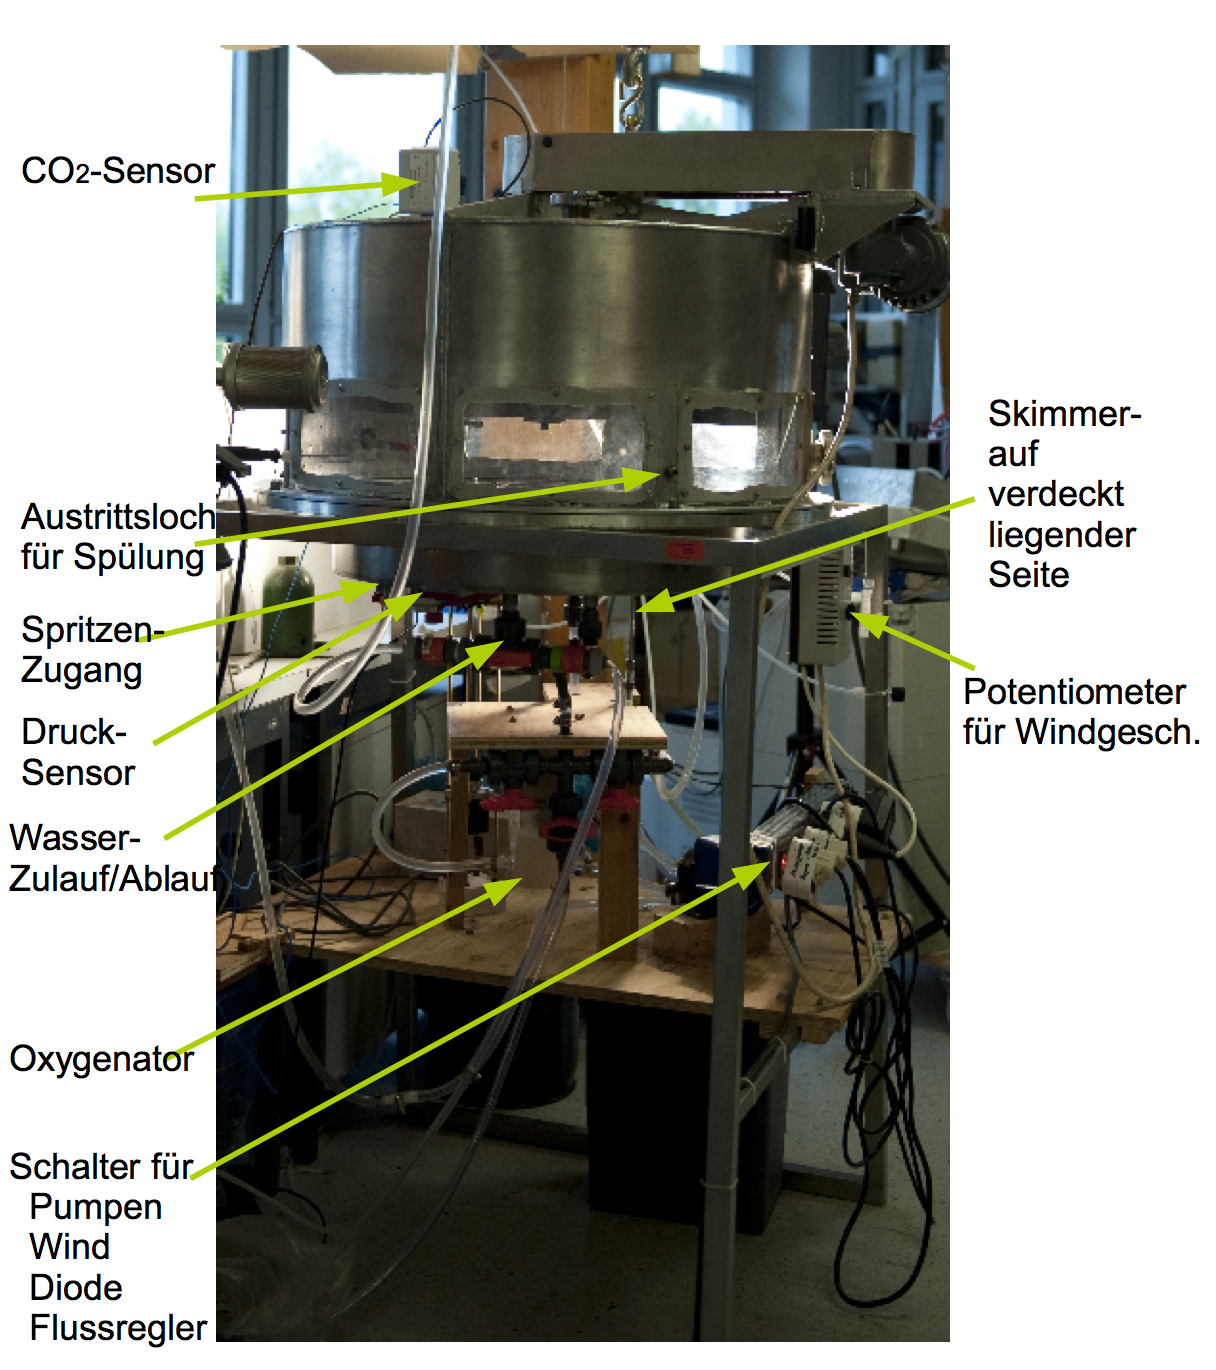
\includegraphics[width=70mm]{Versuchsaufbau}
	\caption{Übersicht über den Versuchsaufbau (Abbildung 10 \cite{jaehne})}
\end{figure}

Wie in der Übersicht zu sehen ist, wird der Versuch in einem ringförmigen Wind-Wellen-Kanal durchgeführt. Für beide Versuchsteile wird vollentsalztes Wasser verwendet. Hierbei handelt es sich um normales Haushaltswasser, was zusätzlich noch mit einem Ionentauscher aufbereitet wurde. Die Füllhöhe der Wasserrinne wird während des Versuchs mit einem Drucksensor über den hydrostatischen Druck gemessen. Der Luftraum wird ständig mit $CO_2$-freier Luft aus einem Reinstluftgenerator gespült. Dies führt zu einem leichten Unterdruck im Kanal, was in der Folge dazu führt, dass keine verunreinigte Umgebungsluft einströmen kann. Temperatur und $CO_2$-Konzentration werden mit handelsüblichen Sonden aufgenommen und vom PC ausgelesen. Für die Erzeugung des Windes stehen vier motorbetriebene Rotorblätter zur Verfügung. Diese kreisen im Luftraum. Über die Motorleistung kann die Windgeschwindigkeit reguliert werden. Der auch im Versuchsaufbau eingezeichnete Oxygenator dient dazu das Wasser mit Gas, in diesem Fall $CO_2$, anzureichern. Seine Funktionsweise ähnelt der einer Lunge. Anschließend wichtig zu nennen ist noch der Skimmer, welcher verwendet wird, um einen evtl. auftretenden Oberflächenfilm vom Wasser absaugen zu können.

\section{Versuchsdurchf\"uhrung}

Zunächst ist anzumerken, dass der Versuch grundsätzlich zwei mal durchgeführt wurde. Das jeweils verwendete Wasser war einmal VE-Wasser und im zweiten Teil Meermodellwasser. Zur Symolation des Meerwassers werden $2.5ml$ einer 1-molaren $NaOH$-Lösung in das gesammte im Wasserkanal befindliche Wasservolumen gegeben.
Nachfolgend soll nur auf die wichtigsten Schritte während des Experiments eingegangen werden. Im Versuchsheft wurde handschriftlich Protokoll über die einzelnen Teile geführt:
1. Prüfen der Leitfähigkeit des verwendeten Wassers, um sicherstellen zu können, dass unter einem bestimmten Schwellenwert. 2. Aufnahme von Lampenspektren 3. Für den Versuchsteil mit Meermodellwasser wird Natriumhydroxid dem Wasser hinzugegeben. 4. Begasung des Wassers mit $CO_2$ 5. Evasionsmessung 6. Alkalisches und saures Referenzspektrum aufnehmen, sowie Dunkelspektrum.

\section{Auswertung/Ergebnisse}
\subsection{VE-Wasser}
\subsubsection{Zeitliche Verl\"aufe der Messdaten}

\begin{figure}[H]
	\centering
	% hier schon der komplixiert Fall, dass 2 Bilder nebeneinander gesetzt werden
	\parbox{82.5mm}{
		\centering
		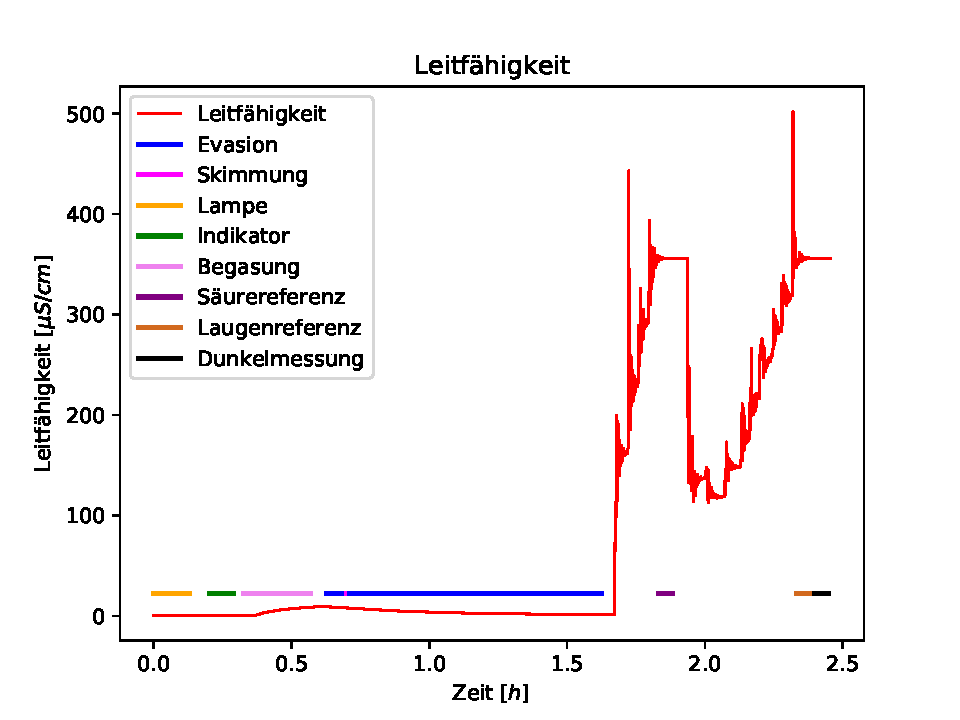
\includegraphics[width=82.5mm]{VE-Wasser/Leitfaehigkeit}
		\caption{Leitf\"ahigkeit}
	}
	\hfill% fuegt Platz ein, das rueckt die beiden Bilder an den Rand
	\parbox{82.5mm}{
		\centering
		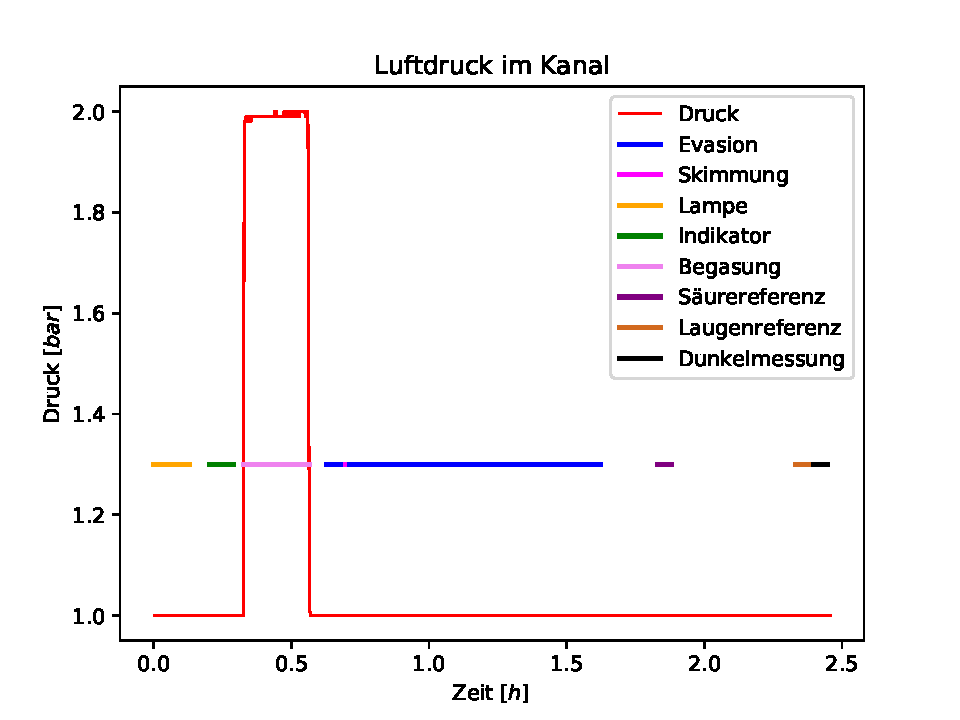
\includegraphics[width=82.5mm]{VE-Wasser/Luftdruck}
		\caption{Luftdruck}
	}
	\centering
	% hier schon der komplixiert Fall, dass 2 Bilder nebeneinander gesetzt werden
	\parbox{82.5mm}{
		\centering
		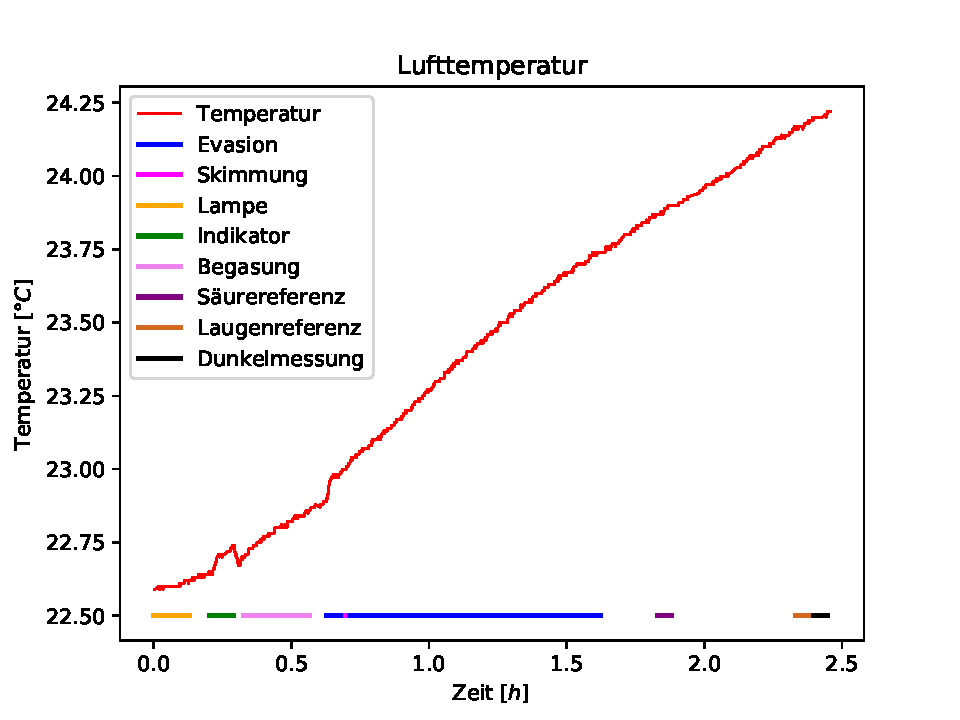
\includegraphics[width=82.5mm]{VE-Wasser/Lufttemperatur}
		\caption{Lufttemperatur}
	}
	\hfill% fuegt Platz ein, das rueckt die beiden Bilder an den Rand
	\parbox{82.5mm}{
		\centering
		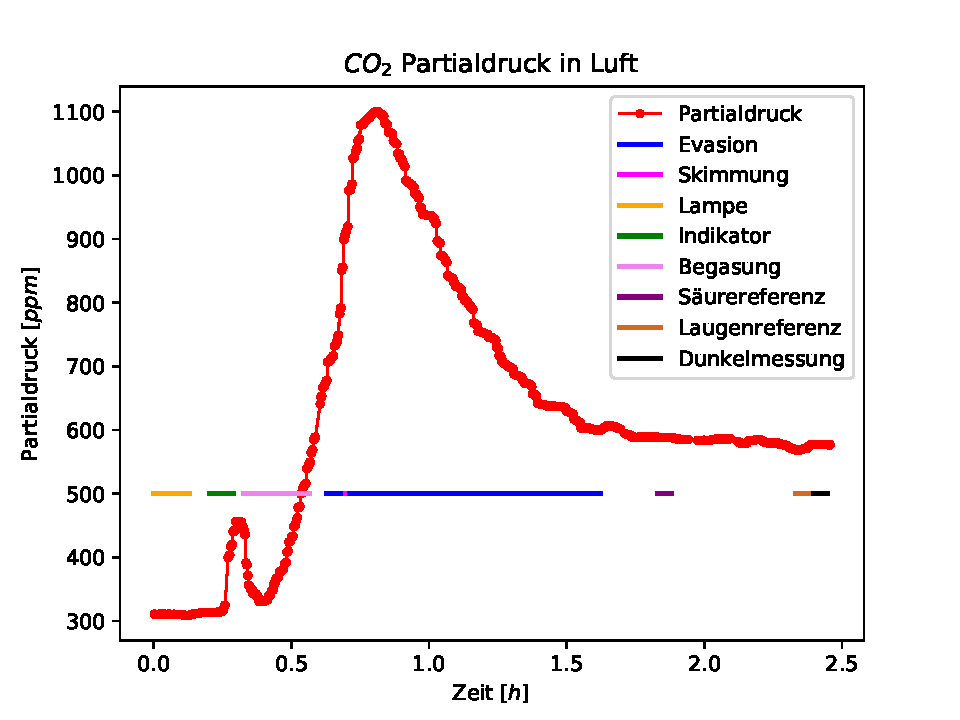
\includegraphics[width=82.5mm]{VE-Wasser/Partialdruck}
		\caption{Partialdruck von $CO_2$}
	}
	\centering
	% hier schon der komplixiert Fall, dass 2 Bilder nebeneinander gesetzt werden
	\parbox{82.5mm}{
		\centering
		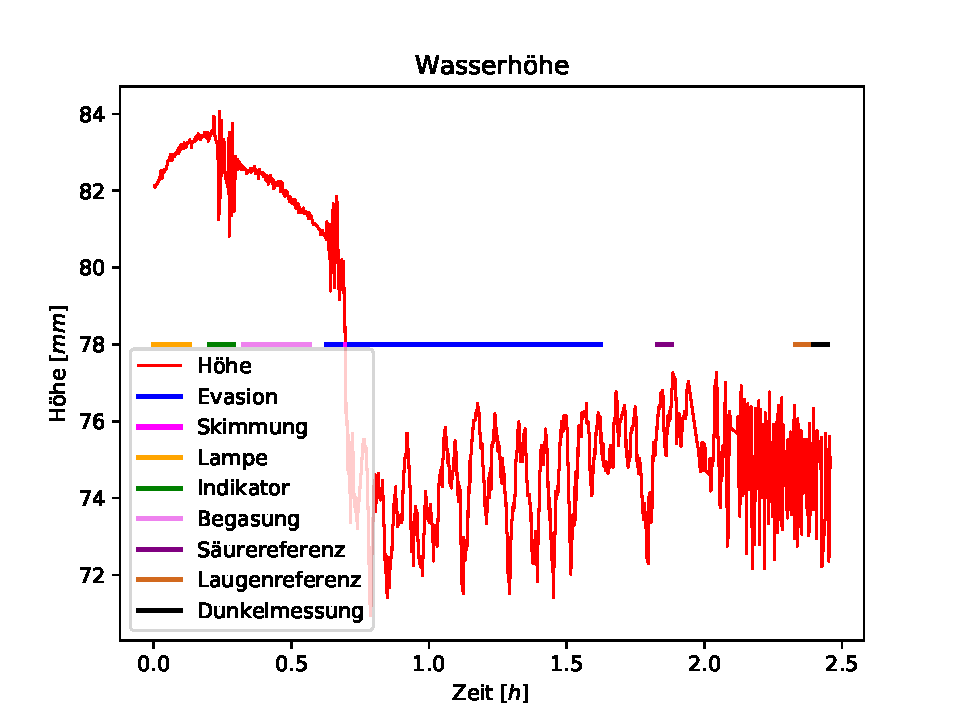
\includegraphics[width=82.5mm]{VE-Wasser/Wasserhoehe}
		\caption{Wasserh\"ohe }
	}
	\hfill% fuegt Platz ein, das rueckt die beiden Bilder an den Rand
	\parbox{82.5mm}{
		\centering
		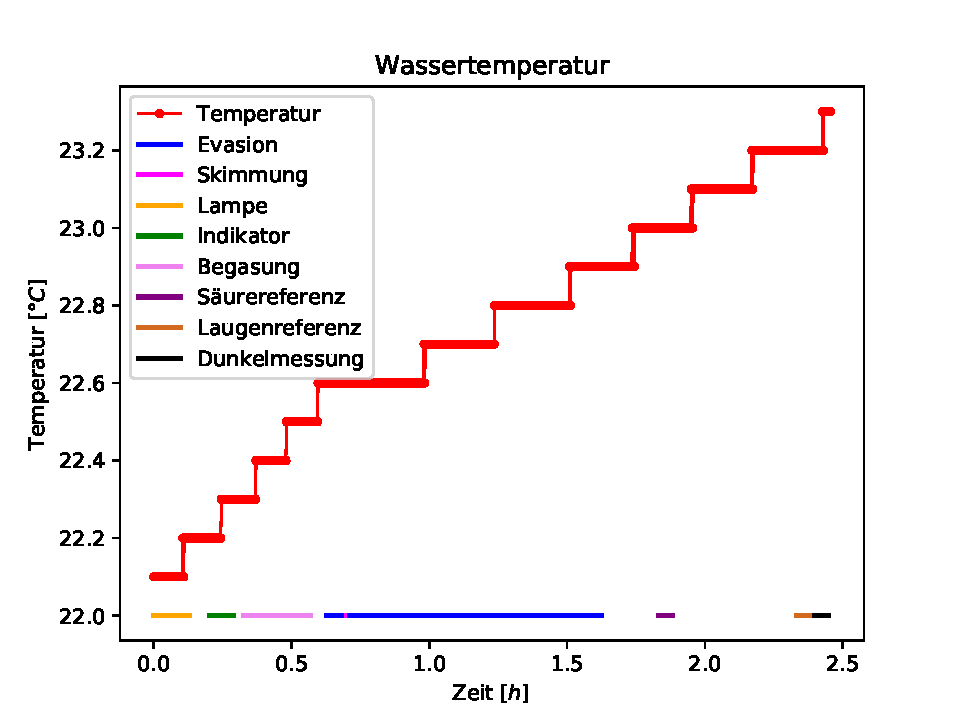
\includegraphics[width=82.5mm]{VE-Wasser/Wassertemperatur}
		\caption{Wassertemperatur }
	}
\end{figure}
\begin{figure}[H]
	\centering
	% hier schon der komplixiert Fall, dass 2 Bilder nebeneinander gesetzt werden
	\parbox{82.5mm}{
		\centering
		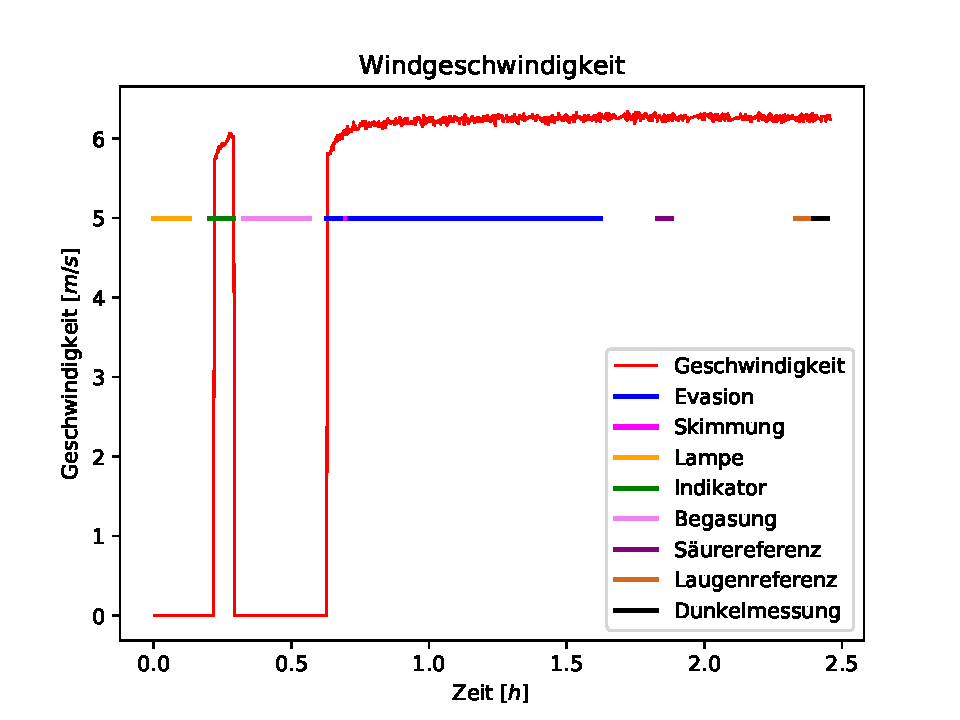
\includegraphics[width=82.5mm]{VE-Wasser/Windgeschwindigkeit}
		\caption{Windgeschwindigkeit}
	}
	\hfill% fuegt Platz ein, das rueckt die beiden Bilder an den Rand
	\parbox{82.5mm}{
		\centering
		%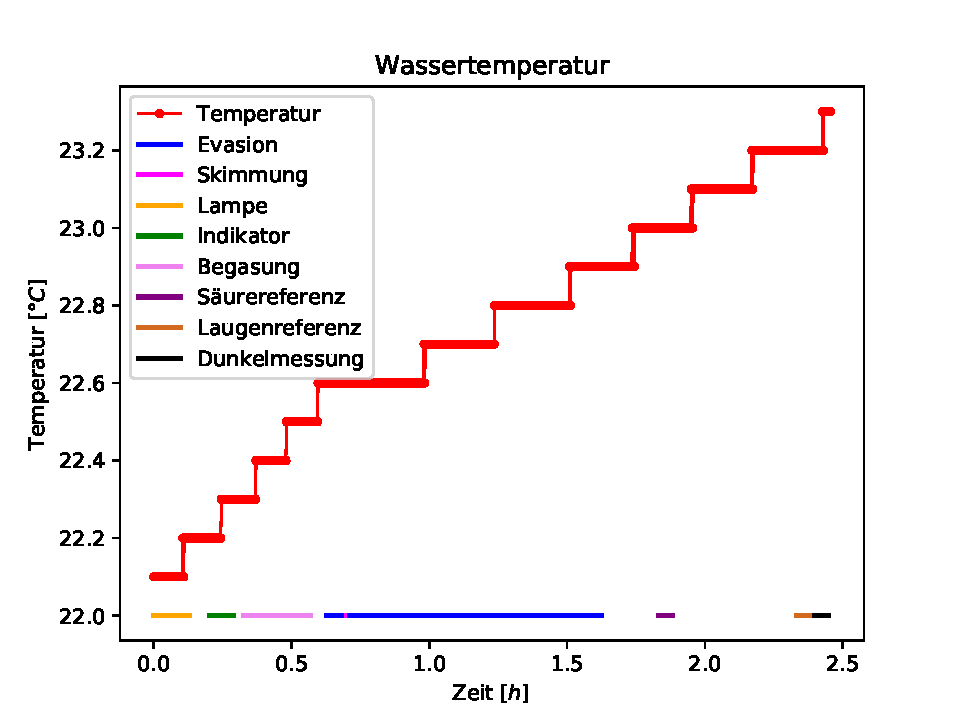
\includegraphics[width=82.5mm]{VE-Wasser/Wassertemperatur}
		%\caption{Wassertemperatur im Wind-Wellen-Kanal \"uber Zeit}
	}
\end{figure}

\subsubsection{Berechnung $CO_2$-Konzentration in Wasser nach Begasung}

Für die Konzentration des gelösten $CO_2$ Gases in Wasser wird zuerst berechnet, mit wieviel Mol an $CO_2$ das Wasser durch den Oxygenator begast wurde. Dazu wird nach folgenden Formeln gerechnet:

\begin{equation}
n = \dot V t \frac{\rho}{M}
\end{equation}

\begin{equation}
\Delta n = \sqrt{(t \frac{\rho}{M} \Delta \dot V)^{2}+(\dot V \frac{\rho}{M} \Delta t)^{2}}
\end{equation}

Mit Dichte: $\rho_{CO_2} = 1.98 \frac{kg}{m^3} $, molarer Masse: $M_{CO_2} = 44.0\frac{g}{mol} $, Zeit:  $t = (867 \pm 8)s$ und Massenfluss: $\dot V = (45.0 \pm 0.1)\frac{ml}{min}$ folgt daraus:

\begin{equation}
n_{w0} = (0.0293 \pm 0.0003) \,mol
\end{equation}

Dieser Wert wird zun\"achst mit dem durch die Löslichkeit von $CO_2$ in Wasser bestimmten Wert verglichen, um absch\"atzen zu können, ob das Wasser w\"ahrend der Begasung schon in S\"attigung war. Das Volumen des Wassers in der Rinne wurde im Skript mit $V = 12.6 \,l $ angegeben. Außerdem ist das Volumen des Leitungssystems von $V=1,1 \,l $ zu ber\"ucksichtigen. Dieses wurde aus Gleichung (44) \cite{jaehne} bestimmt.
\begin{equation}
n = \alpha_{CO_2}(21 °C) \, V = 0.52 \, mol
\end{equation}

Hierbei wurde der Wert für die L\"oslichkeit aus Abbildung 4 \cite{jaehne} verwendet. Es kann also angenommen werden, dass sich die komplette begaste Stoffmenge an $CO_2$ in dem Wasser gelöst hat. Daraus ergibt sich für die anfängliche Konzentration:
\begin{equation}
c_{w0} = \frac{n}{V} = (2.11 \pm 0.02)\cdot 10^{-3} \frac{mol}{l}
\end{equation}

\subsubsection{Untersuchung Boxmodell-Bedingung}

\underline{Frage:} Zu welchen Zeiten im Evasionsexperiment ist die Annahme $c_a \ll c_w/\alpha $ für das einfache Boxmodell erfüllt? \\ \\

\paragraph{Leitfähigkeitsmethode\\}

Zuerst folgt aus der Annahme $\Lambda ^2 \propto c_w $, dass $\Lambda ^2 = m \cdot c_w $. Danach wird also die Konstante $m$ gemäß
\begin{equation}
m = \frac{\Lambda^2(0)}{c_w(0)} = \frac{\Lambda^2(0)}{c_{w0}} = 37456 \frac{(\mu S)^2 l}{cm^2 mol} = 37.5 * 10^-6 \frac{S^2 cm^2}{mol}
\end{equation}
bestimmt. Hierbei wurde (5) zur Berechung verwendet. Mit Hilfe dieser Konstanten kann nun $c_w$ für beliebige Zeiten berechnet und, geteilt durch die Löslichkeit (siehe Abbildung 4 \cite{jaehne}), über die Zeit aufgetragen werden. Trägt man in demselben Diagramm auch den gemessenen Partialdruck von $CO_2$ auf und verwendet eine logarithmische Skalierung, so lässt sich die Größenordnung erkennen, die zwischen $c_a$ und $\frac{c_w}{\alpha}$ liegt.

\begin{figure}[H]
	\centering
	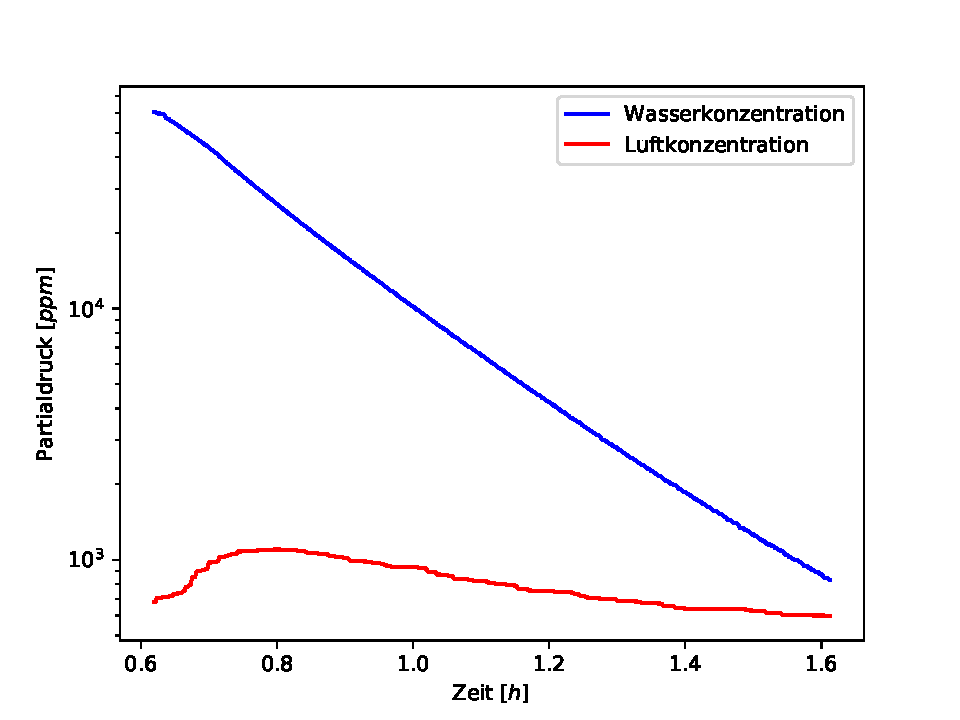
\includegraphics[width=120mm]{VE-Wasser/LeitfaehigkeitQuadrat.pdf}
	\caption{Plot zur Abschätzung der Konzentrationsverhältnisse während Evasion}
\end{figure}

Es ist zu erkennen, dass vor allem zu Beginn der Evasion die Bedingung $c_a \ll c_w/\alpha $ für das einfache Boxmodell deutlich erfüllt ist, es liegen hier beinahe 2 Größenordnungen zwischen den Konzentrationen (Faktor 100). Gegen Ende, man könnte auch schon ab der Hälfte der Evasion sagen, je nach dem, wie streng die Ungleichung zu betrachten ist, wird die Bedingung für das Boxmodell zunehmend nicht mehr erfüllt. Es liegt hier nur noch weniger als eine Größenordnung zwischen den Konzentrationen. \\\\
Eine Anmerkung ist an dieser Stelle noch zu machen. Die Messung des Partialdrucks von $CO_2$ weist mit ungefähr 170 ppm einen realtiv großen Offset auf. Dieser wurde hier jedoch nicht beachtet, da er für die qualitative Aussage keinen Unterschied macht.

\paragraph{Indikatormethode\\}

Auch für diese Methode wird eine Annahme über eine Proportionalität verwendet: $(\frac{[HI]}{[I^-]})^2 \propto c_w $, sodass $(\frac{[HI]}{[I^-]})^2 = m \cdot c_w $. Danach wird also die Konstante $m$ gemäß
\begin{equation}
m = \frac{(\frac{[HI]}{[I^-]})^2(0)}{c_w(0)} = \frac{(\frac{[HI]}{[I^-]})^2(0)}{c_{w0}}
\end{equation}
bestimmt. Des Weiteren sollen verschiedene Verhältnisse $\frac{[HI]}{[I^-]}$, die mit Hilfe des Heurisko-Skripts für verschiedene Wellenlängenbereiche bestimmt wurden, untersucht werden:

\begin{figure}[H]
	\centering
	% hier schon der komplixiert Fall, dass 2 Bilder nebeneinander gesetzt werden
	\parbox{57.5mm}{
		\centering
		\begin{tabular}{c|c|c}
			$\lambda_1 [nm] - \lambda_2 [nm]$ & $\frac{[HI]}{[I^-]}(0)$ & $k [\frac{l}{mol}]$ \\ \hline
			284 - 836 & 2.51 & 2986 \\
			288 - 432 & 2.70 & 3455 \\
			524 - 880 & 2.49 & 2938 \\
			596 - 796 & 2.37 & 2662 \\
			304 - 376 & 2.75 & 3584
		\end{tabular}
		\caption{Tabelle der verschiedenen $\frac{[HI]}{[I^-]}$ und m für unterschiedliche Wellenlängenbereiche}
	}
	\hfill% fuegt Platz ein, das rueckt die beiden Bilder an den Rand
	\parbox{95mm}{
		\centering
		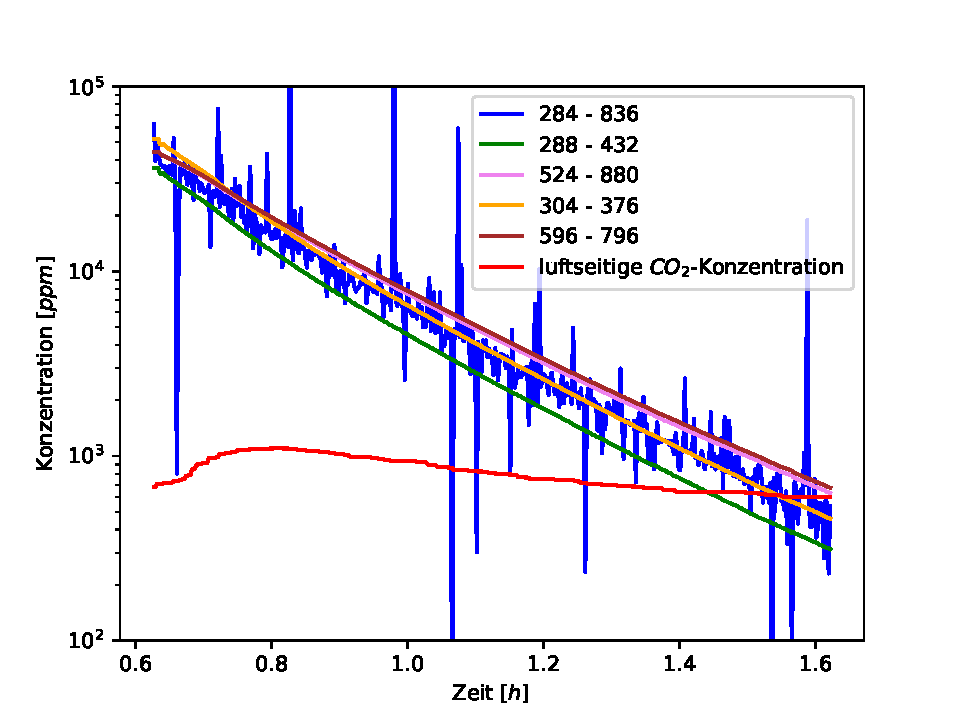
\includegraphics[width=95mm]{VE-Wasser/Indikator.pdf}
		\caption{Plot zur Abschätzung der Konzentrationsverhältnisse während Evasion für verschiedene $\frac{[HI]}{[I^-]}$ bzw. m}
	}
\end{figure}

Grundsätzlich liefert diese Methode die selben Ergebnisse, wie bereits die Leitfähigkeitsmethode. Deshalb soll nur auf die Unterschiede, welche aus den verschiedenen $\frac{[HI]}{[I^-]}$ bzw. verwendeten Wellenlängenbereichen resultieren, eingegangen werden. Es ist zu erkennen, dass die Verwendung eines sehr großen Bereichs des Spektrums zu starken Verrauschungen führt, was vor allem daran liegt, dass auch die grünen Wellenlängen, also der sensible Umschlagsbereich des Indikators verwendet wird. Abgesehen davon scheint der verwendete Wellenlängenbereich keinen großen Einfluss auf die Bewertung der Annahme zu haben, die oben beschriebene Aussage bleibt allgemein gültig.\\
Wichtig an dieser Stelle noch anzumerken ist, dass auch hier, wie im Folgenden (bei Meermodellwasser), der Offset der Luftkonzentrationsmessung nicht berücksichtigt wurde, da nur qualitative Aussagen gemacht werden sollen. Dies erklärt auch, warum die Konzentration im Wasser gegen Ende der Evasion scheinbar unter die in der Luft fällt. Es sollte sich hier maximal ein Gleichgewicht einstellen. Durch das fehlende Offset lässt sich dies jedoch erklären.

\subsubsection{Bestimmung Transfergeschwindigkeit}

Ähnlich wie bei der Leitfähigkeitsmethode zur Abschätzung der Boxmodell-Bedingung wird auch dieses mal der Zusammenhang $\Lambda ^2 \propto c_w $ verwendet. Zusätzlich fließt in die Berechnung auch noch
\begin{equation}
c_w(t) = c_w(0) \cdot exp(-\frac{k}{h_{eff}}t)
\end{equation}
mit ein, was aus Gleichung (42) \cite{jaehne} entnommen wurde. Hierbei entspricht $k$ der gesuchten Transfergescwindigkeit und $h_{eff}$ der effektiven Wasserhöhe, welche aus der gemessenen Wasserhöhe und dem Wasservolumen im Rohrsystem nach (43) und (44) \cite{jaehne} bestimmt wurde. Es ergibt sich also insgesamt folgender Zusammenhang:
\begin{equation}
k = -2 \frac{ln(\Lambda (t)/\Lambda (0))}{t} \cdot h_{eff}
\end{equation}
Das Verhältnis der Leitfähigkeiten muss also logarithmisch geplottet werden, sodass aus der Steigung des Graphen die Transfergeschwindigkeit bestimmt werden kann. Es wurden an dieser Stelle zwei Fits durchgeführt, einmal wurde direkt über den kompletten Zeitbereich eine Exponentialfunktion angepasst und beim zweiten Fit schrittweise für zwei Bereiche und dann die Transfergeschwindigkeit gemittelt.

\begin{figure}[H]
	\centering
	% hier schon der komplixiert Fall, dass 2 Bilder nebeneinander gesetzt werden
	\parbox{82.5mm}{
		\centering
		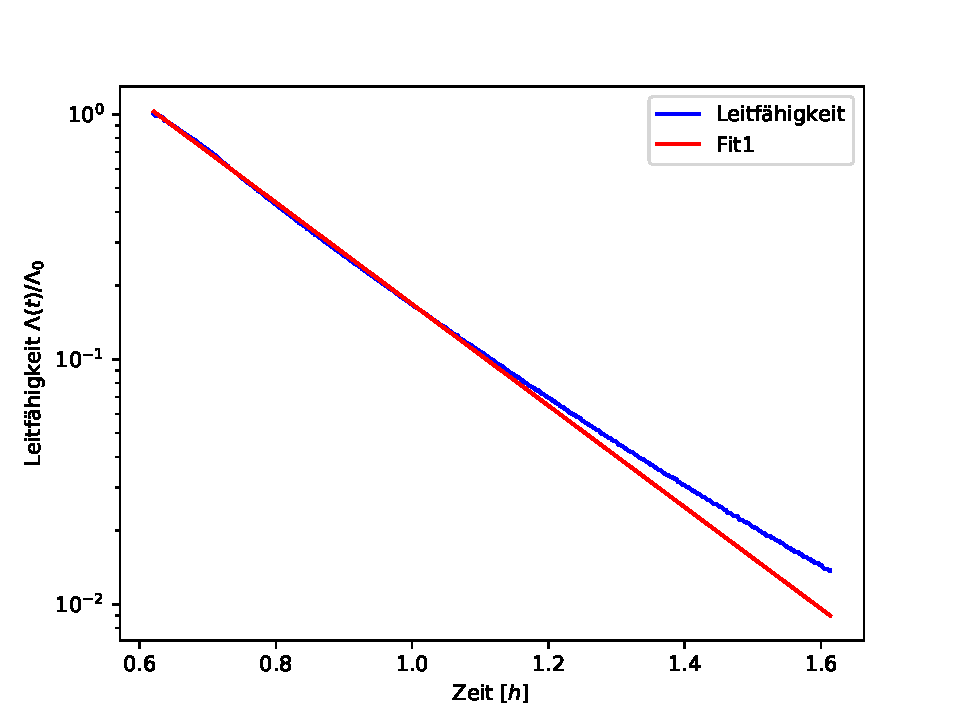
\includegraphics[width=82.5mm]{VE-Wasser/TransferGeschw}
		\caption{Durchgängiger Fit}
	}
	\hfill% fuegt Platz ein, das rueckt die beiden Bilder an den Rand
	\parbox{82.5mm}{
		\centering
		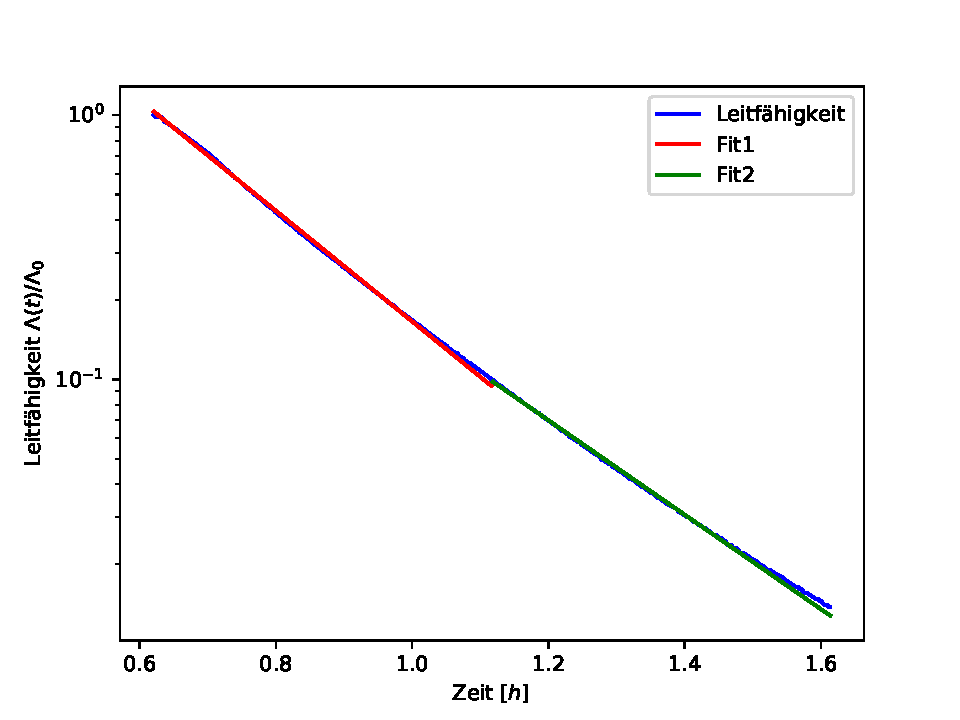
\includegraphics[width=82.5mm]{VE-Wasser/TransferGeschwKnick}
		\caption{Schrittweiser Fit (Halbierung der Fitbreite)}
	}
\end{figure}

 Es ergibt sich für den durchgängigen Fit:

\begin{equation}
	k = (38.9 \pm 0.8)\, \frac{cm}{h}
\end{equation}

Für den schrittweisen Fit folgt:

\begin{equation}
k_{ges} = (36.4 \pm 0.9)\, \frac{cm}{h}
\end{equation}

Hierfür wurden die stückweise berechneten Transfergeschwindigkeiten gemittelt:

\begin{equation}
k_1 = (39.2 \pm 0.8)\, \frac{cm}{h}
\end{equation}

\begin{equation}
	k_2 = (33.6 \pm 0.5)\, \frac{cm}{h}
\end{equation}

Zur besseren Bewertung der Ergebnisse wurden noch die Mittelwerte und Standardabweichungen der Windgeschwindigkeit und der Wassersäule für die verschiedenen Fitbereiche berechnet. Die mittlere quadratische Neigung der Wellen konnte nicht gemessen werden, da das dafür vorgesehene Messgerät nicht funktionstüchtig war.

\paragraph{Durchgängiger Fit}
\begin{itemize}
	\item Wind: $v_w [\frac{m}{s}] = 6.22 \pm 0.06 $
	\item Wassersäule $h_w[mm] = 81.4 \pm 1.6 $
\end{itemize}
\paragraph{Schrittweiser Fit: Teil 1}
\begin{itemize}
	\item Wind: $v_w [\frac{m}{s}] = 6.19 \pm 0.06 $
	\item Wassersäule $h_w[mm] = 81.2 \pm 1.6 $
\end{itemize}
\paragraph{Schrittweiser Fit: Teil 2}
\begin{itemize}
	\item Wind: $v_w [\frac{m}{s}] = 6.26 \pm 0.03 $
	\item Wassersäule $h_w[mm] = 81.6 \pm 1.2 $
\end{itemize}

\subsubsection{Plot der Spektren}

Mit Hilfe der Daten aus der Vorauswertung des Spektren-Bildes, welche mit dem Heurisko-Skript gemacht wurde, wurden die sauren und basischen Referenzspektren, sowie das Lampen- und das Dunkelspektrum geplottet:

\begin{figure}[H]
	\centering
	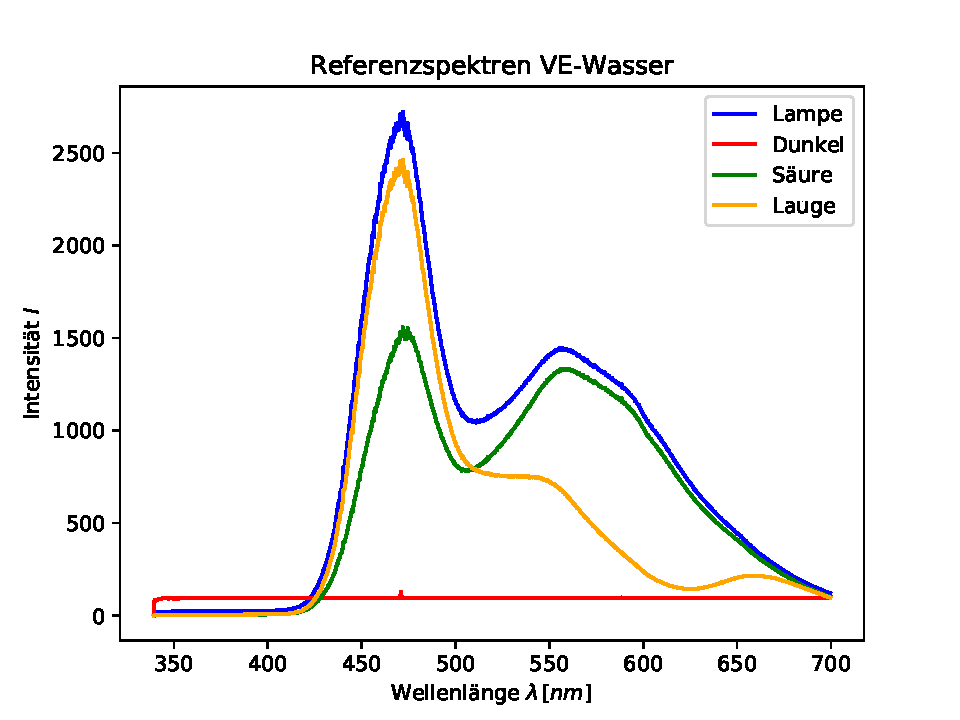
\includegraphics[width=120mm]{VE-Wasser/Referenzspektren}
	\caption{Plot der Spektren für VE-Wasser}
\end{figure}

\subsubsection{Bestimmung Transfergeschwindigkeit - $\frac{[HI]}{[I^-]}$ Methode}
\begin{figure}[H]
	\centering
	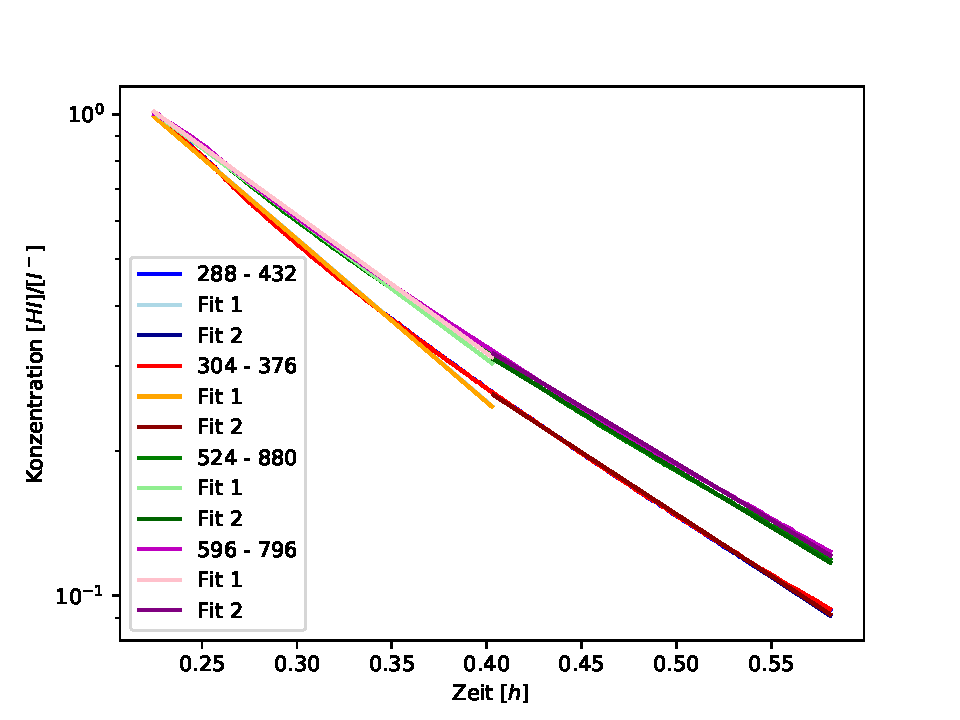
\includegraphics[width=120mm]{VE-Wasser/TransferhIKnick}
	\caption{Plot der Konzentrationen $\frac{[HI]}{[I^-]}$ über Zeit für verschiedene Wellenlängen mit Fits (Trennung bei $t \approx 0.4h$)}
\end{figure}

Aus der Steigung des Graphen wird nun wieder die Transfergeschwindigkeit nach Gleichung (8) und der Annahme $(\frac{[HI]}{[I^-]})^2 \propto c_w $ bestimmt.
Daraus folgt für die Geschwindigkeit (siehe oben):
\begin{equation}
k = -2 \frac{ln(\frac{[HI]}{[I^-]}(t)/\frac{[HI]}{[I^-]}(0))}{t} \cdot h_{eff}
\end{equation}

Die einzelnen Transfergeschwindigkeiten, welche aus den Fits aus der ersten Hälfte des Graphen ermittelt wurden, werden mit denen der zweiten Hälfte zu dem Wert $k_{ges} \, [\frac{cm}{h}]$ gemittelt.

\begin{figure}[H]
	\centering
	\begin{tabular}{c|c|c|c}
		Wellenlängenbereich $[nm]$ & $k_1 [\frac{cm}{h}]$ & $k_2 [\frac{cm}{h}]$ & $k_{ges} [\frac{cm}{h}] $ \\ \hline
		288 - 432 & $47.1 \pm 1.4$ & $35.2 \pm 0.5$ & $41.2 \pm 1.5$ \\
		304 - 376 & $47.2 \pm 1.4$ & $35.0 \pm 0.5$ & $41.1 \pm 1.5$ \\
		524 - 880 & $39.9 \pm 1.2$ & $32.5 \pm 0.5$ & $36.2 \pm 1.3$ \\
    	596 - 796 & $39.0 \pm 1.2$ & $32.2 \pm 0.5$ & $35.6 \pm 1.3$
	\end{tabular}
	\caption{Transfergeschwindigkeiten für unterschiedliche Wellenlängenbereiche}
\end{figure}

Zur besseren Bewertung der Ergebnisse wurden noch die Mittelwerte und Standardabweichungen der Windgeschwindigkeit und der Wassersäule für die verschiedenen Fitbereiche berechnet. Die mittlere quadratische Neigung der Wellen konnte nicht gemessen werden, da das dafür vorgesehene Messgerät nicht funktionstüchtig war.

\paragraph{Teil 1}
\begin{itemize}
	\item Wind: $v_w [\frac{m}{s}] = 6.1 \pm 0.5 $
	\item Wassersäule $h_w[mm] = 81.7 \pm 2.5 $
\end{itemize}
\paragraph{Teil 2}
\begin{itemize}
	\item Wind: $v_w [\frac{m}{s}] = 6.25 \pm 0.03 $
	\item Wassersäule $h_w[mm] = 81.5 \pm 1.2 $
\end{itemize}

\subsection{Meermodellwasser}
\subsubsection{Zeitliche Verl\"aufe der Messdaten}

\begin{figure}[H]
	\centering
	% hier schon der komplixiert Fall, dass 2 Bilder nebeneinander gesetzt werden
	\parbox{82.5mm}{
		\centering
		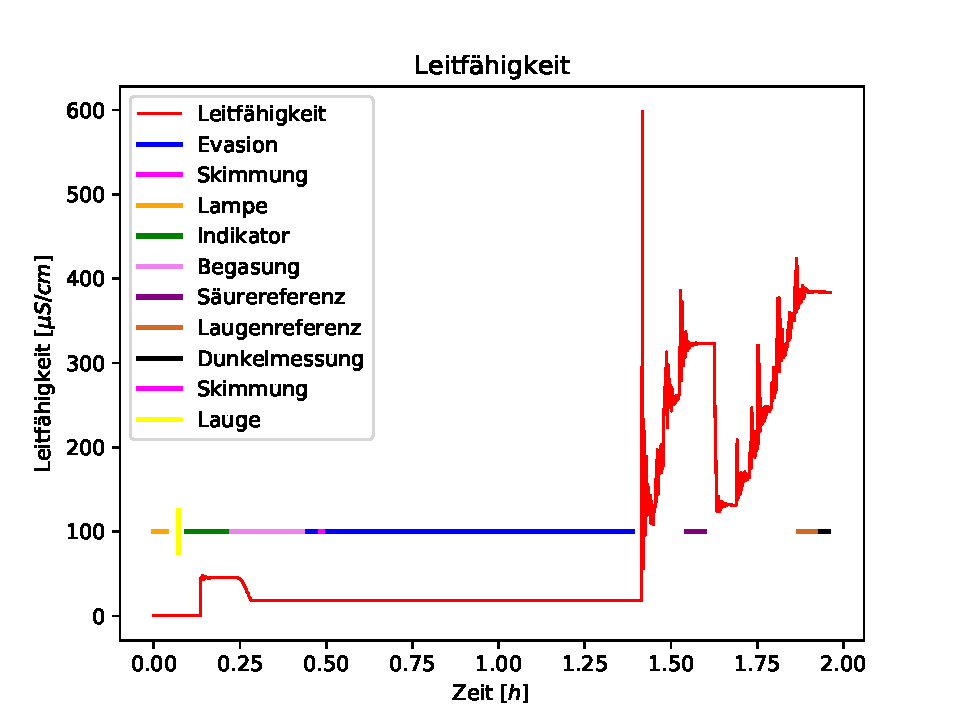
\includegraphics[width=82.5mm]{Meerwasser/Leitfaehigkeit}
		\caption{Leitf\"ahigkeit}
	}
	\hfill% fuegt Platz ein, das rueckt die beiden Bilder an den Rand
	\parbox{82.5mm}{
		\centering
		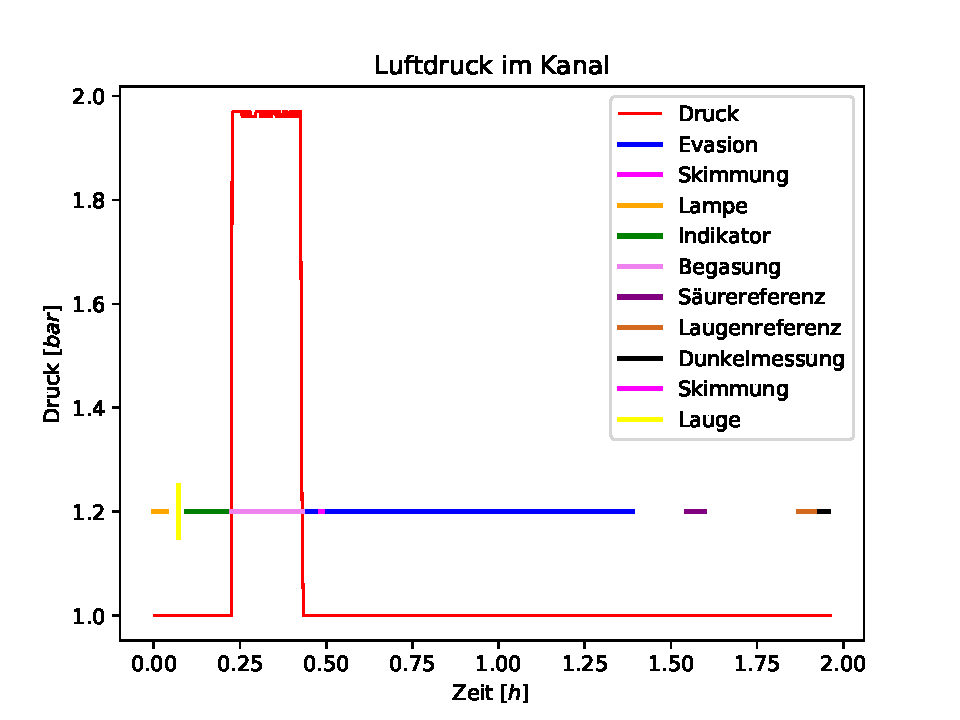
\includegraphics[width=82.5mm]{Meerwasser/Luftdruck}
		\caption{Luftdruck}
	}
	\centering
	% hier schon der komplixiert Fall, dass 2 Bilder nebeneinander gesetzt werden
	\parbox{82.5mm}{
		\centering
		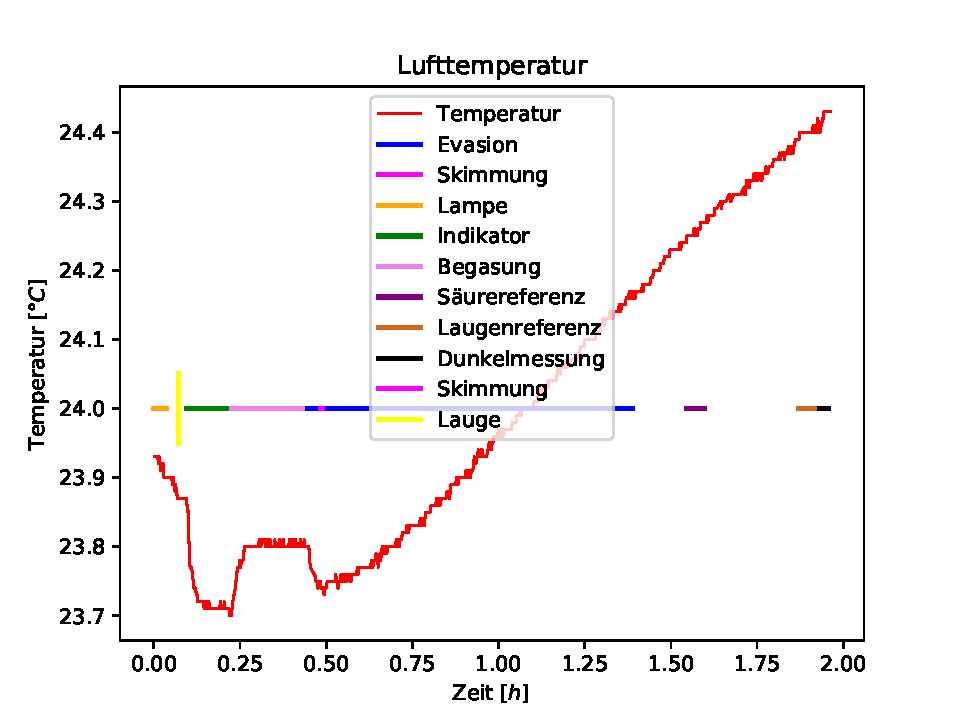
\includegraphics[width=82.5mm]{Meerwasser/Lufttemperatur}
		\caption{Lufttemperatur}
	}
	\hfill% fuegt Platz ein, das rueckt die beiden Bilder an den Rand
	\parbox{82.5mm}{
		\centering
		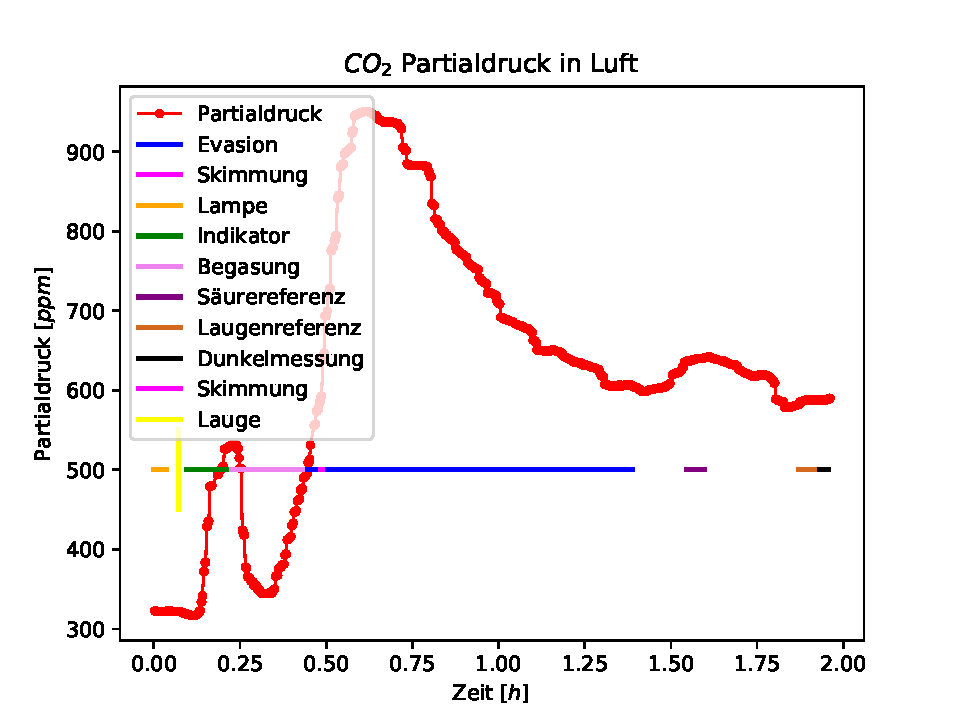
\includegraphics[width=82.5mm]{Meerwasser/Partialdruck}
		\caption{Partialdruck von $CO_2$}
	}
	\centering
	% hier schon der komplixiert Fall, dass 2 Bilder nebeneinander gesetzt werden
	\parbox{82.5mm}{
		\centering
		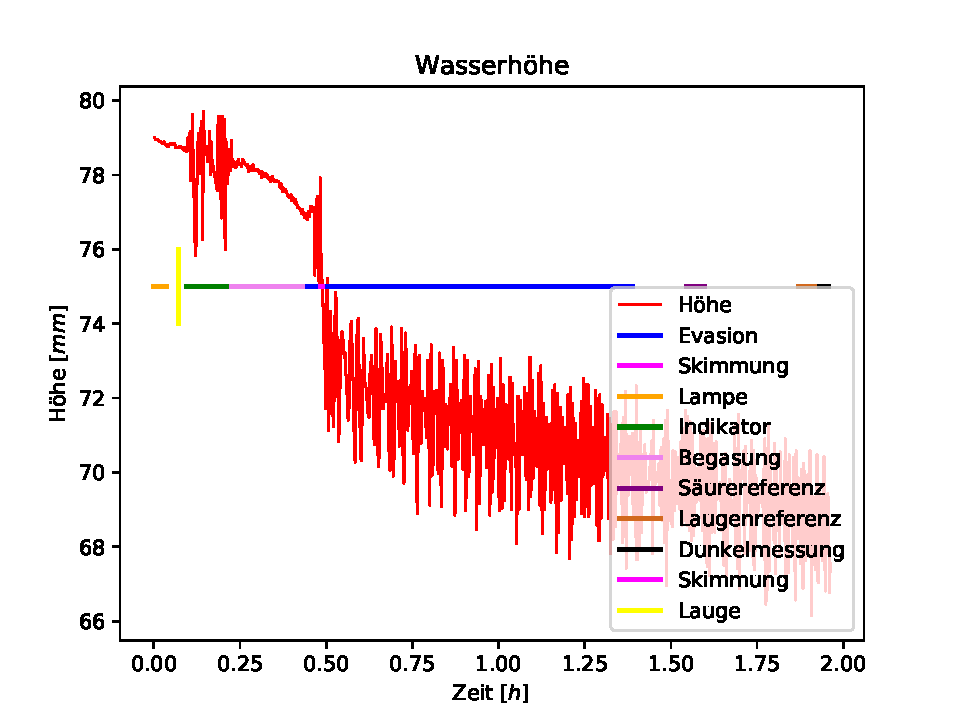
\includegraphics[width=82.5mm]{Meerwasser/Wasserhoehe}
		\caption{Wasserh\"ohe }
	}
	\hfill% fuegt Platz ein, das rueckt die beiden Bilder an den Rand
	\parbox{82.5mm}{
		\centering
		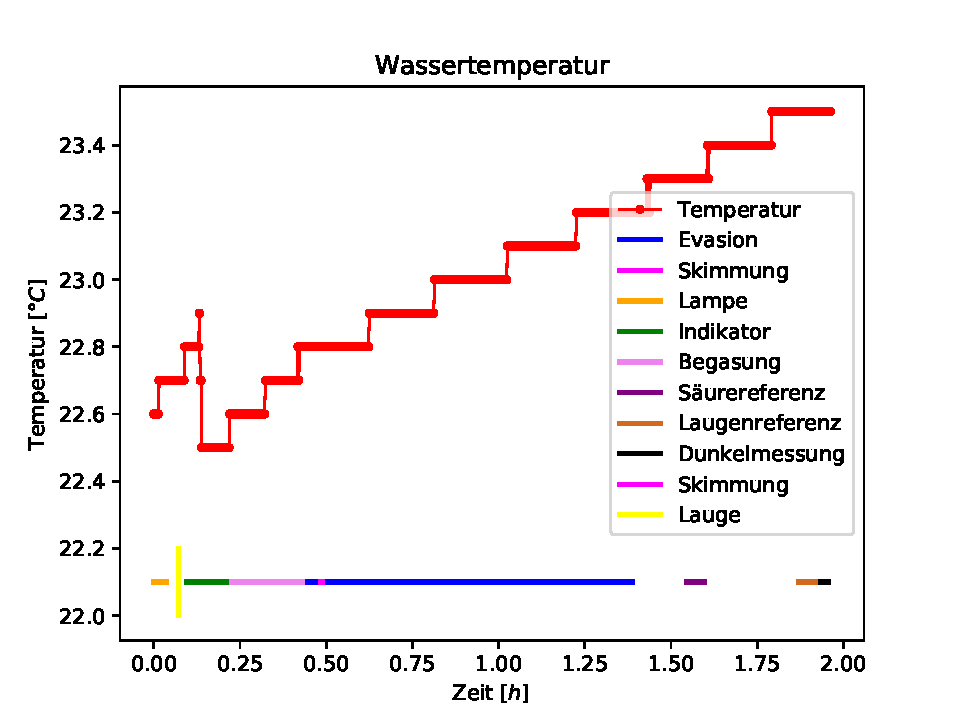
\includegraphics[width=82.5mm]{Meerwasser/Wassertemperatur}
		\caption{Wassertemperatur }
	}
\end{figure}
\begin{figure}[H]
	\centering
	% hier schon der komplixiert Fall, dass 2 Bilder nebeneinander gesetzt werden
	\parbox{82.5mm}{
		\centering
		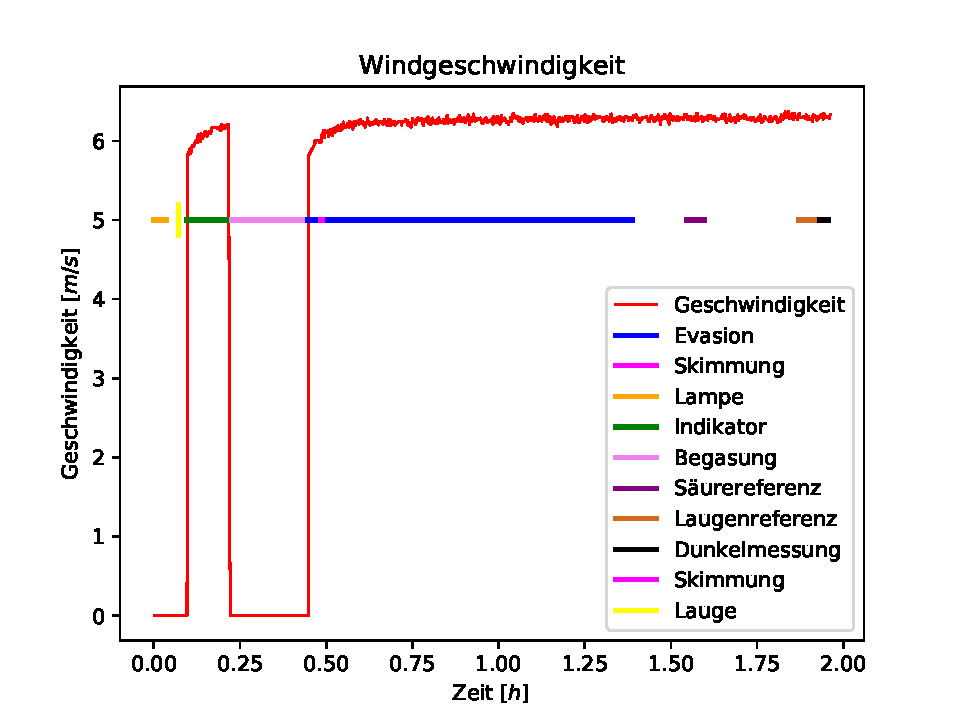
\includegraphics[width=82.5mm]{Meerwasser/Windgeschwindigkeit}
		\caption{Windgeschwindigkeit}
	}
	\hfill% fuegt Platz ein, das rueckt die beiden Bilder an den Rand
	\parbox{82.5mm}{
		\centering
		%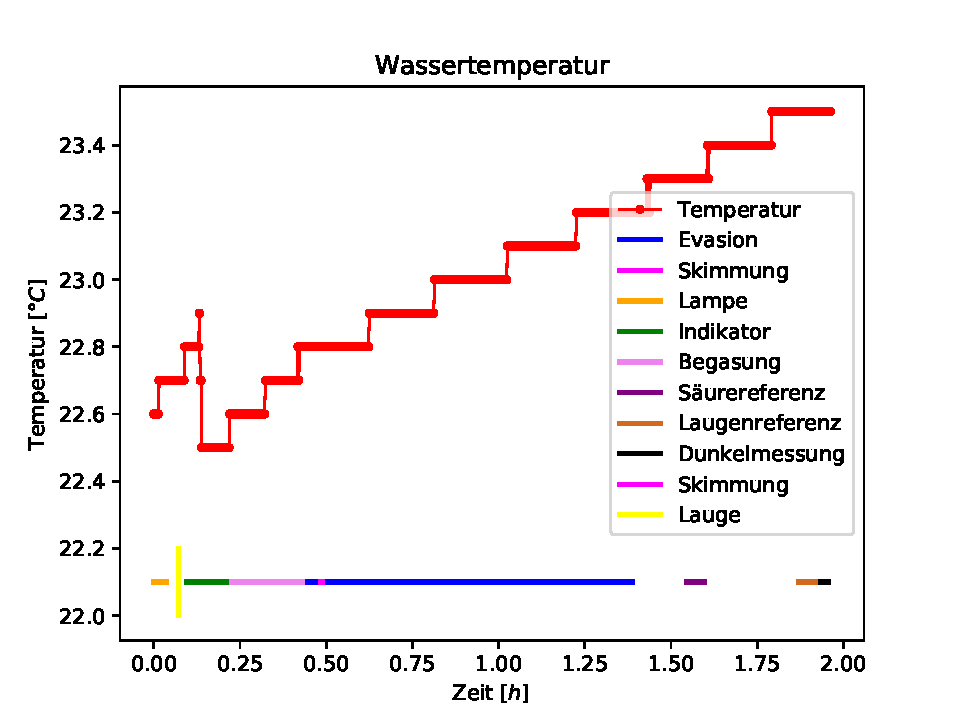
\includegraphics[width=82.5mm]{Meerwasser/Wassertemperatur}
		%\caption{Wassertemperatur im Wind-Wellen-Kanal \"uber Zeit}
	}
\end{figure}

%% Bilder: Sie sollten nicht versuchen, postscript 'from scratch' selbst zu
%% schreiben, sondern den Output von Analyseroutinen (PAW, ROOT, ...) oder
%% von Plot-Programmen (xfig, tgif) verwenden

\subsubsection{Berechnung $CO_2$-Konzentration in Wasser nach Begasung}

Für die Konzentration des gelösten $CO_2$ Gases in Wasser wird zuerst berechnet, mit wieviel Mol an $CO_2$ das Wasser durch den Oxygenator begast wurde. Dazu wird nach folgenden Formeln gerechnet:

\begin{equation}
n = \dot V t \frac{\rho}{M}
\end{equation}

\begin{equation}
\Delta n = \sqrt{(t \frac{\rho}{M} \Delta \dot V)^{2}+(\dot V \frac{\rho}{M} \Delta t)^{2}}
\end{equation}

Mit Dichte: $\rho_{CO_2} = 1.98 \frac{kg}{m^3} $, molarer Masse: $M_{CO_2} = 44.0\frac{g}{mol} $, Zeit:  $t = (737 \pm 8)s$ und Massenfluss: $\dot V = (45.0 \pm 0.1)\frac{ml}{min}$ folgt daraus:

\begin{equation}
n_{w0} = (0.0249 \pm 0.0003) \,mol
\end{equation}

Dieser Wert wird zun\"achst mit dem durch die Lösbarkeit von $CO_2$ in Wasser bestimmten Wert verglichen, um absch\"atzen zu können, ob das Wasser w\"ahrend der Begasung schon in S\"attigung war. Das Volumen des Wassers in der Rinne wurde im Skript mit $V = 12.6 \,l $ angegeben. Außerdem ist das Volumen des Leitungssystems von $V=1,1 \,l $ zu ber\"ucksichtigen. Dieses wurde aus Gleichung (44) \cite{jaehne} bestimmt.
\begin{equation}
n = \alpha_{CO_2}(21 °C) \, V = 0.52 \, mol
\end{equation}

Hierbei wurde der Wert für die L\"oslichkeit aus Abbildung 4 \cite{jaehne} verwendet und es wurde davon ausgegangen, dass sich diese durch die Zugabe von Natronlauge in das VE-Wasser nicht wesentlich geändert hat. Es kann also angenommen werden, dass sich die komplette begaste Stoffmenge an $CO_2$ in dem Wasser gelöst hat. Daraus ergibt sich für die anfängliche Konzentration:
\begin{equation}
c_{w0} = \frac{n}{V} = (1.82 \pm 0.02)\cdot 10^{-3} \frac{mol}{l}
\end{equation}

\subsubsection{Untersuchung Boxmodell-Bedingung}

\underline{Frage:} Zu welchen Zeiten im Evasionsexperiment ist die Annahme $c_a \ll c_w/\alpha $ für das einfache Boxmodell erfüllt? \\ \\

\paragraph{Indikatormethode\\}

Für diese Methode wird eine Annahme über eine Proportionalität verwendet: $\frac{[HI]}{[I^-]} \propto c_w $, sodass $\frac{[HI]}{[I^-]} = m \cdot c_w $. Danach wird also die Konstante $m$ gemäß
\begin{equation}
m = \frac{\frac{[HI]}{[I^-]}(0)}{c_w(0)} = \frac{\frac{[HI]}{[I^-]}(0)}{c_{w0}}
\end{equation}
bestimmt. Des Weiteren sollen verschiedene Verhältnisse $\frac{[HI]}{[I^-]}$, die mit Hilfe des Heurisko-Skripts für verschiedene Wellenlängenbereiche bestimmt wurden, untersucht werden: \\

\begin{figure}[H]
	\centering
	% hier schon der komplixiert Fall, dass 2 Bilder nebeneinander gesetzt werden
	\parbox{57.5mm}{
		\centering
		\begin{tabular}{c|c|c}
			$\lambda_1 [nm] - \lambda_2 [nm]$ & $\frac{[HI]}{[I^-]}(0)$ & $m [\frac{l}{mol}]$ \\ \hline
			252 - 760 & 8.52 & 4681 \\
			264 - 368 & 10.37 & 5697 \\
			596 - 796 & 6.63 & 3643 \\
			496 - 764 & 7.25 & 3984 \\
			548 - 644 & 7.48 & 4110
		\end{tabular}
		\caption{Tabelle der verschiedenen $\frac{[HI]}{[I^-]}$ und m für unterschiedliche Wellenlängenbereiche}
	}
	\hfill% fuegt Platz ein, das rueckt die beiden Bilder an den Rand
	\parbox{95mm}{
		\centering
		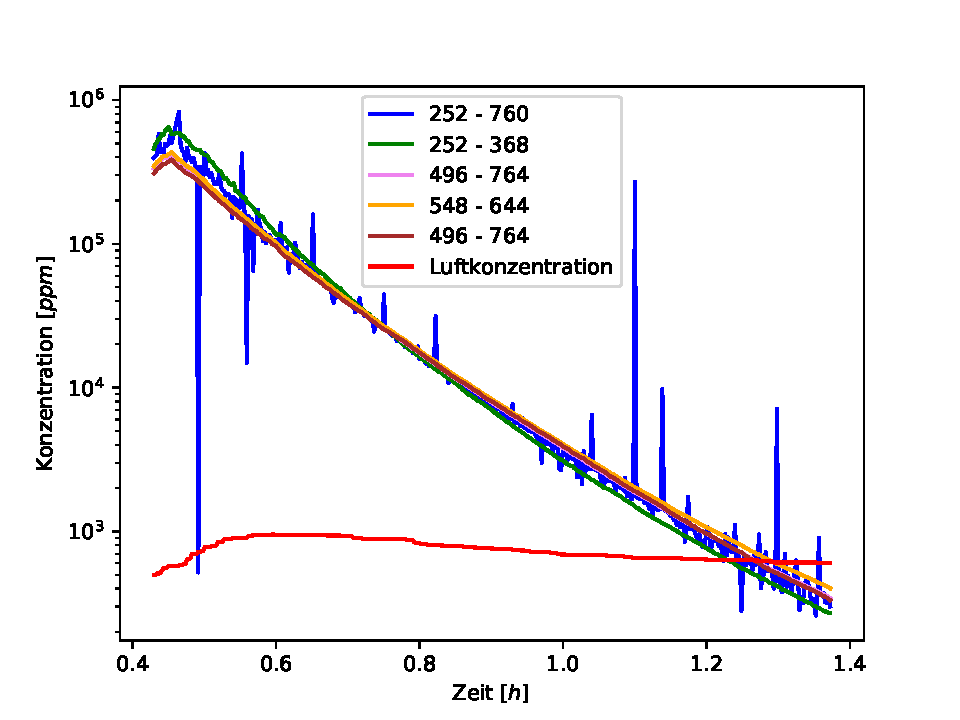
\includegraphics[width=95mm]{Meerwasser/Indikator.pdf}
		\caption{Plot zur Abschätzung der Konzentrationsverhältnisse während Evasion für verschiedene $\frac{[HI]}{[I^-]}$ bzw. m}
	}
\end{figure}

Es ist zu erkennen, dass vor allem zu Beginn der Evasion die Bedingung $c_a \ll c_w/\alpha $ für das einfache Boxmodell deutlich erfüllt ist, es liegen hier beinahe 2 Größenordnungen zwischen den Konzentrationen (Faktor 100). Gegen Ende, man könnte auch schon ab der Hälfte der Evasion sagen, je nach dem, wie streng die Ungleichung zu betrachten ist, wird die Bedingung für das Boxmodell zunehmend nicht mehr erfüllt. Es liegt hier nur noch weniger als eine Größenordnung zwischen den Konzentrationen. Zu beachten ist auch, dass die Verwendung eines großen Wellenlängenbereichs zu einer starken Verrauschung der Konzentration führt. Dies liegt auch hier wieder an dem sensiblen Umschlagsbereich, der mit einbezogen wird. Unterschiede zwischen den anderen Wellenlängenbereichen sind kaum zu erkennen.\\\
Für die Anmerkungen zu dem Offset der Luftkonzentration siehe oben.

\subsubsection{Plot der Spektren}

Mit Hilfe der Daten aus der Vorauswertung des Spektren-Bildes, welche mit dem Heurisko-Skript gemacht wurde, wurden die sauren und basischen Referenzspektren, sowie das Lampen- und das Dunkelspektrum geplottet:

\begin{figure}[H]
	\centering
	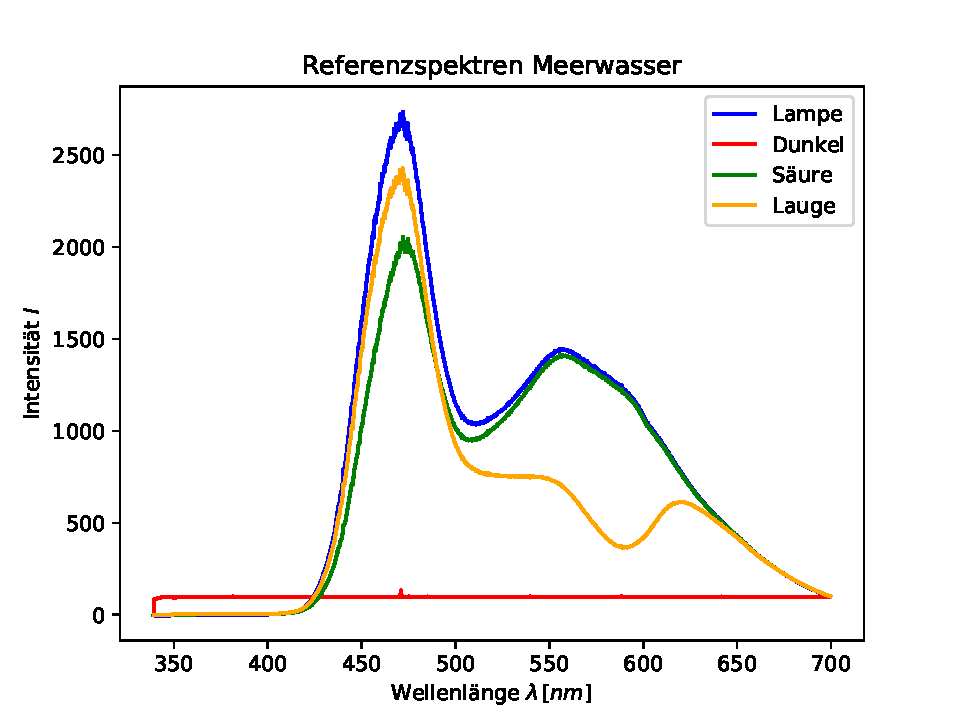
\includegraphics[width=120mm]{Meerwasser/Referenzspektren}
	\caption{Plot der Spektren für das Meermodellwasser}
\end{figure}

\subsubsection{Bestimmung Transfergeschwindigkeit - $\frac{[HI]}{[I^-]}$ Methode}
\begin{figure}[H]
	\centering
	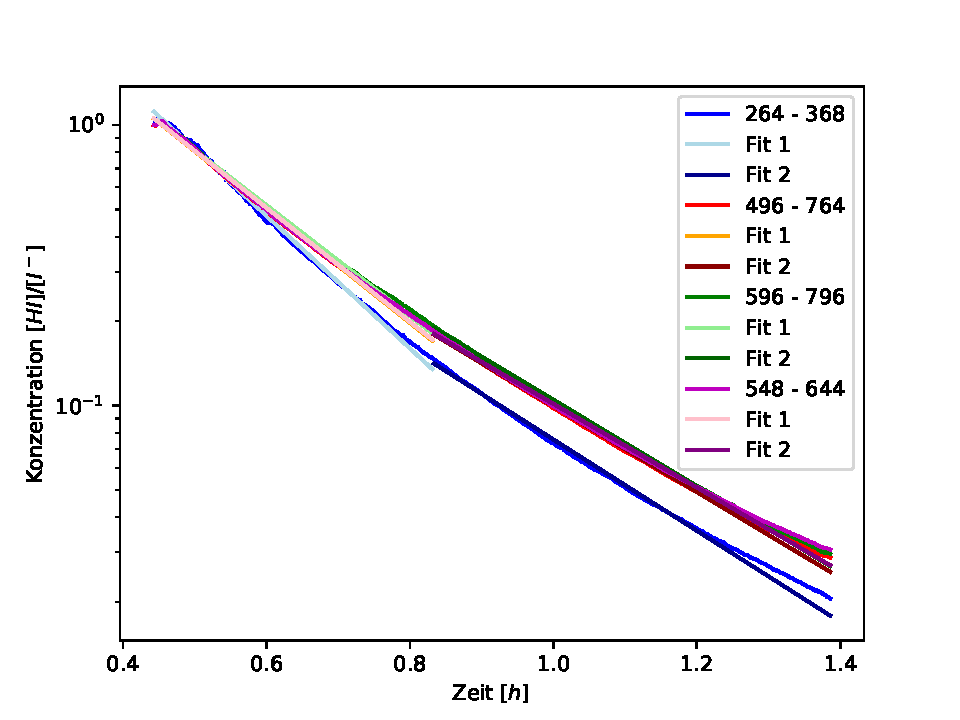
\includegraphics[width=120mm]{Meerwasser/TransferhIKnick}
	\caption{Plot der Konzentrationen $\frac{[HI]}{[I^-]}$ über Zeit für verschiedene Wellenlängen mit Fits (Trennung bei $t \approx 0.83h$)}
\end{figure}

Aus der Steigung des Graphen wird nun wieder die Transfergeschwindigkeit nach Gleichung (8) und der Annahme $\frac{[HI]}{[I^-]} \propto c_w $ bestimmt.
Daraus folgt für die Geschwindigkeit (siehe oben):
\begin{equation}
k = - \frac{ln(\frac{[HI]}{[I^-]}(t)/\frac{[HI]}{[I^-]}(0))}{t} \cdot h_{eff}
\end{equation}

Die einzelnen Transfergeschwindigkeiten, welche aus den Fits aus der ersten Hälfte des Graphen ermittelt wurden, werden mit denen der zweiten Hälfte zu dem Wert $k_{ges} \, [\frac{cm}{h}]$ gemittelt.

\begin{figure}[H]
	\centering
	\begin{tabular}{c|c|c|c}
		Wellenlängenbereich $[nm]$ & $k_1 [\frac{cm}{h}]$ & $k_2 [\frac{cm}{h}]$ & $k_{ges} [\frac{cm}{h}] $ \\ \hline
		264 - 368 & $43.2 \pm 1.0$ & $29.1 \pm 0.5$ & $36.2 \pm 1.1$ \\
		496 - 764 & $37.3 \pm 0.8$ & $27.3 \pm 0.4$ & $32.3 \pm 0.9$ \\
		596 - 796 & $36.1 \pm 0.8$ & $27.4 \pm 0.4$ & $31.8 \pm 0.9$ \\
		548 - 644 & $37.1 \pm 0.8$ & $26.7 \pm 0.4$ & $31.9 \pm 0.9$
	\end{tabular}
	\caption{Transfergeschwindigkeiten für unterschiedliche Wellenlängenbereiche}
\end{figure}

Zur besseren Bewertung der Ergebnisse wurden noch die Mittelwerte und Standardabweichungen der Windgeschwindigkeit und der Wassersäule für die verschiedenen Fitbereiche berechnet. Die mittlere quadratische Neigung der Wellen konnte nicht gemessen werden, da das dafür vorgesehene Messgerät nicht funktionstüchtig war.

\paragraph{Teil 1}
\begin{itemize}
	\item Wind: $v_w [\frac{m}{s}] = 6.1 \pm 0.8 $
	\item Wassersäule $h_w[mm] = 79.5 \pm 1.8 $
\end{itemize}
\paragraph{Teil 2}
\begin{itemize}
	\item Wind: $v_w [\frac{m}{s}] = 6.27 \pm 0.03 $
	\item Wassersäule $h_w[mm] = 77.6 \pm 1.2 $
\end{itemize}

\section{Diskussion}

% Zeitliche Verläufe der Messdaten
In diesem Versuch sollen vorrangig die Auswirkungen der verschiedenen Umwelteinflüsse auf den Gasaustausch zwischen Ozean und Atmosphäre untersucht werden. In dem für dieses Experiment verwendeten Wind-Wellen-Kanal wurde besonders die Wasserzusammensetzung betrachtet. Andere zu beobachtende Parameter, wie die Windgeschwindigkeit, der Oberflächenfilm oder auch die Wasserhöhe konnten nahezu konstant gehalten werden (Abbildungen 2-8, 17-23).

Die zeitlichen Verläufe der Messdaten zwischen beiden Messungen unterscheiden sich kaum. Am meisten ähnelt sich der Luftdruck, wobei zwischen Abbildung 3 und 18 nicht nur der Verlauf gleich ist, sondern sogar die absoluten Zahlenwerte. Dies kommt daher, dass der atmosphärische Luftdruck sehr stabil ist und nur bei einem starken Wetterumschwung leicht seinen Wert ändert. Da der Kanal nicht luftdicht verschlossen war, sondern mehrere Luftlöcher existierten, konnte sich der Druck ungehindert auch innerhalb des Experiments einstellen.
Der abrupte Anstieg des Drucks passiert zeitgleich mit Einsetzen der Begasung, was logischerweise durch das zusätzlich einströmende Gas zu erklären ist. Während des Prozesses ist der Druck nicht konstant. Dies rührt von einer leichten Schwankung in der Flussrate des $CO_2$ und somit wahrscheinlich von den statistischen Änderungen der Ausflussgeschwindigkeit des Gases aus der Gasflasche und der dahinter geschalteten Druckminderung her.
Fast genauso ähneln sich die Abbildungen 8 und 23 für die Windgeschwindigkeiten. Der Ventilator für die künstliche Erzeugung des Winds wurde durch einen Elektromotor gesteuert und kannte dabei nur zwei Zustände: Wind an / Wind aus. Die Geschwindigkeit war zwar einstellbar, doch wurde sie für die Versuchsdauer konstant gelassen. Zu sehen ist noch ein zeitlich verzögertes Erreichen der eingestellten Windgeschwindigkeit nach Einschalten des Ventilators.
Zur Schonung des Materials wurde der Propeller nicht sofort auf die gewünschte Geschwindigkeit hochgefahren, sondern erhöhte langsam seine Drehfrequenz. Zudem ist zu beachten, dass der Ventilator unabhängig von der Windmessung war und somit die tatsächliche Windgeschwindigkeit gemessen wurde. Diese kann sich nicht instantan auf die Geschwindigkeit des Propellers anpassen, sondern die Bewegungsänderung muss sich erst nach und nach durch die Luftschichten ausbreiten. Somit registriert das Potentiometer auch die langsame Anpassung der Luftbewegung an den Ventilator.

Bei Betrachtung der Temperaturen bietet es sich an, neben den Messungen in beiden Versuchsteilen auch die Wasser- und die Lufttemperatur zu vergleichen (Abbildungen 7 \& 22, 4 \& 19. Abgesehen von kleinen Unsicherheiten am Anfang der Abbildungen 19 \& 22 sieht man eindeutig, dass alle vier Kurven linear ansteigen.
Der Anstieg der Lufttemperatur wird hauptsächlich durch die Abwärme des Ventilatormotors hervorgerufen, was in der kleinen Luftkammer bereits einen nicht unerheblicher Einfluss darstellt.
Die Graphen der Wassertemperatur zeigen einen stufenartigen Anstieg, der durch die ungenaue Datenaufzeichnung der Messwerte zu erklären ist. Dadurch sind zwar feine Schwankungen der Wassertemperatur nicht zu sehen, aber der allgemeine Trend ist klar ersichtlich. Zu erklären ist dieses Wachstum mit dem aus der Hausleitung stammenden VE-Wasser. Es ist generell kühler als die Raumtemperatur und steht bei der Evasionsmessung im Kanal, wo es ins thermische Gleichgewicht mit der Lufttemperatur gelangen will, sprich sich erwärmt.

Die gemessene Wasserhöhe schwankt am meisten in beiden Versuchsteilen (Abbildungen 6 \& 21), was auch durchaus so gewollt ist. Durch den eingestellten Wind werden innerhalb des Kanals Wellen erzeugt, die die Wassersäule teilweise massiv beeinflussen. Es wurden Wellen von etwa einem Zentimeter Höhe beobachtet, das entspricht bei einer Fülllhöhe von etwa sieben Zentimetern im Kanal bereits 15\%. Der überwiegende Abfall der Füllhöhe ist eigentlich unerwünscht und durch eine undichte Stelle im Versuchsaufbau zu begründen. Es entwich über den ganzen Messungszeitraum Flüssigkeit aus dem Kanal, was nicht wieder hinzugegeben wurde.

Der Partialdruck von $CO_2$ im Wasser ist in den Abbildungen 5 \& 20 zu sehen. Er hängt direkt mit den am Experiment durchgeführten Eingriffen zusammen, die durch die horizontalen Balken eingezeichnet sind. So ist etwa der größte Anstieg gefolgt von dem exponentiellen Abfall die verzögerte Reaktion auf die Begasung des Wassers mit sofortiger Evasion des $CO_2$ in die Luft. Der Abfall ist dann so zu erklären, dass durch die sinkende Gaskonzentration im Wasser auch der abzugebende Teil an $CO_2$ an die Luft kleiner wird. Dadurch senkt sich der Partialdruck des Gases insgesamt.
Der kleinere Hochpunkt zu Beginn beider Messreihen ist mit \cite{jaehne} Abb. 8
zu verstehen. So ist die $CO_2$-Konzentration im VE-Wasser nie ganz null, da durch den Ionentauscher nur geladene Teilchen herausgefiltert werden können. Gelöst liegen aber $CO_2, CO_3^{2-} $ und $HCO_3^-$ vor, wovon $CO_2$ Moleküle nicht geladen sind und in Lösung bleiben.
Dieser Anteil evasiert in die anfangs stehende Luft, der Partialdruck steigt. Nach dem Anschalten des Ventilators gelangt frische, gereinigte Luft in das Experiment und der $CO_2$ Anteil in Luft sinkt wieder auf den Anfangswert bis die Begasung wirksam wird.

Die Leitfähigkeitsmessungen zeigen in Abb. 2 \& 17 erst nach der Evasionsmessungen starke Schwankungen, was besonders durch die Zugabe von $HCl$ und $NaOH$ bewirkt wird. Dadurch befinden sich plötzlich viel mehr Ionen im Kanal, die durch die Messmethode registriert werden. Die Zugaben erfolgten jeweils Schrittweise, was auch den gezackten Anstieg in den Plots erklärt.
Der Abfall zwischen den beiden Peaks, der wieder in beiden Abbildungen vorkommt, zeigt die Neutralisation von Salzsäure mit Natronlauge, also die Bindung der Ionen zu ungeladenen Molekülen, ehe weiter Lauge hinzugegeben wird. Auch danach ist während der Messung eine konstante Menge Ionen vorhanden, was die Leitfähigkeit nicht ändert.

Zu dem Versuchs- bzw. Auswertungsteil zur Bestimmung der Anfangskonzentration von $CO_2$ nach Beendigung der Begasung sollen an dieser Stelle noch einmal einige Dinge angemerkt werden. Zunächst wurde sowohl bei VE-, als auch bei Meermodellwasser die Menge an begastem $CO_2$ berechnet. Hierbei wurde der auf 21°C normierte Massenfluss verwendet, da wir nicht die exakte Temperatur des Gases, als es in den Oxygenator gelangt ist, bestimmen konnten. Auch wenn die Lufttemperatur mit ca. 23°C darüber lag, nehmen wir an, dass das Gas aus der Flasche etwas kühler war, weshalb die Normtemperatur gut passen sollte. Zur Abschätzung, ob sich auch das gesamte Gas im Wasser gelöst hat, erschien es sinnvoll zu bestimmen, wieviel Gas sich potentiell in dem Wasser lösen kann. Hierfür wurde die Löslichkeit für 21°C verwendet, was auch kein Problem darstellt, denn diese verändert sich über die Temperatur nicht so sehr, dass sie die Abschätzung signifikant beeinflussen würde. Außerdem ist zu erkennen, dass die Menge an begastem $CO_2$ deutlich unter der potentiell Lösbaren liegt. Daraus resultiert unsere Annahme, dass sämtliches Gas auch tatsächlich im Wasser gelöst wurde. Dies führt uns auf die beiden Anfangskonzentrationen von $c_{w0} = (2.11 \pm 0.02)\cdot 10^{-3} \frac{mol}{l}$ (VE-Wasser) und $c_{w0} = (1.82 \pm 0.02)\cdot 10^{-3} \frac{mol}{l}$ (Meermodellwasser). Die unterschiedlichen Werte ergeben sich vor allem aus den unterschiedlich langen Begasungszeiten. Es wurde von uns angenommen, dass die Zugabe von NaOH bei Meermodellwasser die Löslichkeit des Gases nicht signifikant ändert. Die Werte für die Anfangskonzentrationen erscheinen sinnvoll, denn sie fließen später in die Berechung der Transfergeschwindigkeiten mit ein und führen dort auf Werte, welche mit der Literatur übereinstimmen.

Zu der Beurteilung der Boxmodellbedingung $c_a \ll c_w/\alpha $ während der Evasionsmessung ist hier auch noch etwas anzumerken, auch wenn die wesentlichen Ergebnisse bereits oben präsentiert und kommentiert wurden. Die unterschiedlichen Anfangskonzentrationen bei Beginn der Evasion für die unterschiedlichen Wasser ergeben sich aus den unterschiedlichen Zeiten, die zwischen Begasung und Evasion lagen. Diese war bei VE-Wasser nämlich höher, was zu einem größeren, bereits ausgegasten Teil an $CO_2$ geführt hat. Die Berechnungen mit Hilfe der beiden Methoden bei VE-Wasser und mit Hilfe der Indikatormethode bei Meermodellwasser liefern qualitativ die selben Aussage, was auch unseren Erwartungen entspricht. Auch ergeben sich keine großen Unterschiede zwischen der Indikator- und der Leitfähigkeitsmethode, was dafür spricht, dass diese in gleichem Maße für nachfolgende Berechnungen geeignet sind. Große Unterschiede zwischen den verwendeten Wellenlängenbereichen ergeben sich, abgesehen von den Wellenlängen die der Farbe des Indikators im Umschlagpunkt entsprechen, kaum. Hier treten starke Verrauschungen auf, was auf die Sensibilität (schnelle Farbänderung) des Indikators in diesem Bereich zurückzuführen ist. Wichtig abschließend noch zu erwähnen ist, dass die Boxmodell-Bedingung ab ungefähr Mitte der Evasion nicht mehr gültig ist. Trotzdem wurde sie in den weiteren Rechungen als über die ganze Zeit gültig erachtet. Dies könnte auch als potentielle Fehlerquelle für nachfolgende Ergebnisse angeführt werden. In jedem Fall ist zu sehen, dass sich in beiden Teilversuchen, die mit Hilfe der Indikatormethode schrittweise bestimmten Transfergeschwindigkeiten für die beiden Zeiträume stark unterscheiden.

Im nächsten Schritt wurde mit der Leitfähigkeitsmethode nur die Transfergeschwindigkeit für VE-Wasser bestimmt. Die Methode ist auf Meermodellwasser aufgrund der zustätzlich anwesenden Ionen nicht anzuwenden. Die berechneten Transfergeschwindigkeiten von $k = (38.9 \pm 0.8)\, \frac{cm}{h}$ bzw. $k_{ges} = (36.4 \pm 0.9)\, \frac{cm}{h}$ liegen im Bereich der später nach der Indikatormethode bestimmten Werte und auch im Bereich der Literaturwerte (\cite{jaehne} Abb. 6). Die angegebenen Ungenauigkeiten ergeben sich aus den Fits, sind jedoch, vergleicht man das schrittweise mit dem Komplett-Fit Vorgehen, deutlich höher anzusetzen. Das schrittweise Vorgehen erscheint hier deutlich genauer zu sein, was an der Güte der Fits ersichtlich wird. Hier wird der Verlauf deutlich besser beschrieben. Auch unterschiedliche Windgeschwindigkeiten oder Höhen der Wassersäulen könnten für Differenzen gesorgt haben. Vor allem die Windgeschwindigkeiten haben sich gemessen an ihren Ungenauigkeiten stark geändert. Seltsam erscheint jedoch die geringere Transfergeschwindigkeit im zweiten Teil der schrittweisen Methode, auch wenn dort die Windgeschwindigkeit höher war. Umgekehrtes ist nämlich zu erwarten. Vielleicht hat sich in dieser Zeit aber auch ein Oberflächenfilm gebildet, der von uns nicht bemerkt wurde und so für eine Dämpfung gesorgt hat. Mit Daten können wir dies jedoch nicht belegen, da der $mss$ der Wellen nicht gemessen werden konnte, anhand dessen Abnahme dies begründet hätte werden können.

Als nächster Punkt scheint wichtig, die gemessenen Spektren zu kommentieren. Zuerst soll dies für VE-Wasser geschehen. Der Dunkelstrom wurde bestimmt und bei den übrigen Spektren abgezogen. Als Referenzspektrum wurde das Spektrum der Lampe aufgenommen. Anhand dessen lassen sich Unterschiede der sauren und alkalischen Referenzspektren erkennen. Als Indikator wurde in diesem Fall Bromkresolgrün verwendet, welches im Umschlagpunkt grün, im Sauren gelb und im Alkalischen blau ist. All das lässt sich auch in den Referenzspektren erkennen. Der Schnittpunkt der beiden Referenzspektren liegt bei etwa 500 nm, was genau der Farbe des Indikators im Umschlagpunkt entspricht. Hier ist die Lösung sozusagen so sauer wie alkalisch, was sich in der gleich großen Intensität in den Spektren wiederspiegelt. Sowohl bei 470 nm (Blau) als auch ab 550 nm (Gelb) unterscheiden sich die beiden Referenzspektren stark. Hier dominiert jeweils das Spektrum, welches zu dem Milieu gehört, das durch den Indikator angezeigt wird. Entsprechend höher ist die Intensität.
Analoge Aussagen lassen sich für die Spektrenbilder des Meermodellwassers treffen. Hier wurde der Indikator Bromkresolpurpur verwendet, entsprechend ist der Umschlagpunkt eher im Blauen (480 nm) zu erkennen. Hier überwiegt auch das alkalische Referenzspektrum. Umgekehrtes gilt bei höheren Wellenlängen ab 550 nm, wenn auch der Indikator zunehmend rot wurde, was einem sauren Mileu entspricht.

% Bestimmung der Transfergeschwindigkeit
% Vergleich beider Messmethoden
Wie in der Auswertung zu sehen, kann die Transfergeschwindigkeit auf zwei unterschiedliche Arten gemessen werden. Dadurch wird ein Vergleich beider Methoden möglich, was jedoch nur für das VE-Wasser gilt. Eine der beiden benötigten Proportionalitäten gilt nur bei reinem Wasser und somit nicht für das Meermodellwasser.
Im Vergleich der Transfergeschwindigkeiten beider Methoden sieht man, dass der mittels Leitfähigkeit bestimmte Wert genau zwischen den Werten aus der Absorptionsmessung liegt. Hierbei zeigt sich, dass die Absorptionsmessung für verschiedene Wellenlängen recht unterschiedliche Werte liefert. Dabei spielen die später näher betrachteten Parameter, wie Wind und Wassersäule keine Rolle, da die Absorptionsspektren der einzelnen Wellenlängen exakt zu gleichen Zeiten aufgezeichnet wurden.
Durch die Annahme $c_w \propto \frac{[HI]}{[I^-]}$ ist hier nur der verwendete Indikator - Bromkresolgrün - entscheidend. Durch ihn wird das Licht abhängig von der $CO_2$ Konzentration beeinflusst.  Dazu können die Plots Abb. 15 \& 27 betrachtet werden. Auch hier zeigt sich nicht die gleiche Steigung der Geraden in der logarithmischen Darstellung, sondern die Konzentrationsabnahme ändert sich entsprechend der Wellenlängenbereiche. Hierbei ist zu beachten, dass dies vermutlich an den unterschiedlichen Referenzspektren liegt, die als Basis für die Berechung des Verhältnisses $\frac{[HI]}{[I^-]}$ verwendet wurden. Hauptsächlich für höherer Wellenlängen ergibt sich ein im Vergleich zum Lampenspektrum komplett unterschiedlicher Verlauf der Intensität für das alkalische Referenzspektrum. Dies könnte also die Ursache für die unterschiedlichen Transfergeschwindigkeiten sein, die aus $\frac{[HI]}{[I^-]}$ bestimmt werden. Warum das alkalische Referenzspektrum bei hohen Wellenlängen von der Form, wie auch von der Intensität sich so stark von dem Lampenspektrum unterscheidet hat vermutlich chemische Ursachen, auf die hier nicht genauer eingegangen werden kann. Angesprochene Unterschiede können bei Meermodellwasser bis zu beinahe 14\% erreichen, bei VE-Wasser sogar fast 16\%.

% Vergleich beider Wasserzusammensetzungen
Um die Wasserzusammensetzungen und auch die Einflüsse von Ionen im Wasser besser beurteilen zu können, bietet es sich an, die gemessenen Transfergeschwindigkeiten mittels der $\frac{[HI]}{[I^-]}$ Methode zu vergleichen. Dazu werden für die vier betrachteten Wellenlängenbereiche einzeln die Geschwindigkeiten gegenübergestellt.
Für niedrige Wellenlängenbereiche ($\lambda \approx 350 nm$) liegt die Transfergeschwindigkeit für VE-Wasser knapp 14\% höher als für das Meermodellwasser, für hohe Bereiche, also $\lambda \approx 700 nm$ ergibt sich die gleiche Abweichung der Modelle. Das heißt Meerwasser wird durch die zusätzlich vorhandenen Ionen im $CO_2$ Austausch eher gehemmt gegenüber einfachem $H_2O$.
Das macht in sofern Sinn, da $CO_2$ Moleküle in nicht ionisierter Form hauptsächlich in saurem Wasser vorliegen und nicht so sehr in Meerwasser, was in etwa einen pH-Wert von 8 hat.
Man kann diese Werte auch über die ablaufenden Reaktionen von $CO_2$ in Wasser anschauen:
Die Transfergeschwindigkeit ist höher, wenn das Verhältnis $\frac{[HI]}{[I^-]}$ schneller abnimmt. Daraus folgt, dass die Reaktion $HI \, + \, H_2O \rightleftharpoons \, I^- \, + \, H_3O^+$ schneller in die rechte Richtung ablaufen muss. Genau das passiert für neutrales Wasser schneller als für alkalisches Meerwasser.

% Einfluss der Parameter auf die Transfergeschwindigkeiten
Insgesamt kommt bei allen Berechnungen heraus, dass die Transfergeschwindigkeit zu Beginn der Evasionsmessung höher ist als gegen Ende. Dies sollte eigentlich nicht passieren, da die Transfergeschwindigkeit als Quotient aus Netto-Fluss und Konzentrationsdifferenz hier theoretisch konstant ist. Aus Gleichung 1 geht jedoch hervor, dass $k \propto h_{eff}$ gilt.
Wie in den Abbildungen 6 \& 21 zu sehen, nimmt die Wassersäule ab und damit sollte auch die Transfergeschwindigkeit geringer werden, was sie, laut Abb. 15 \& 27, tut.
Ein weiterer Einfluss existiert in dem Anstieg der Temperatur. Er ist über das gesamte Experiment etwa konstant und hat damit laut \cite{jaehne} Abb. 4 eine sinkende Löslichkeit zur Folge. Das wiederum hat einen größeren Einfluss auf die Transfergeschwindigkeit, je weniger die Invasion im Boxmodell mit $c_w \ll \alpha c_a $ vernachlässigt werden kann. Außerdem würde sich, wie ober bereits beschrieben dadurch der gesamte Formalismus ändern.
Auch die betrachtete Windgeschwindigkeit steigt über den Zeitraum der Evasionsmessung an, was ein Indiz für einen dicker werdenden Oberflächenfilm sein kann. Ein dickerer Oberflächenfilm hat dann eine stärker dämpfende Eigenschaft auf den Gasaustausch. Diese Annahme konnte jedoch nicht quantitativ bestätigt werden, da dazu eine funktionsfähige Wellenenigungsmessung nötig gewesen wäre. Mit bloßem Auge waren keine Änderungen des Wellenbildes erkennbar, doch sind bereits geringfügige Änderungen des Oberflächenfilms ausschlaggebend für die Transfergeschwindigkeit.

Letztlich ist die Ungenauigkeit der bestimmten Geschwindigkeiten sicherlich noch höher als in der Auswertung bestimmt. Es wurden hier nur die Standardabweichungen betrachtet, die bei den zugrunde liegenden großen Datensätzen kaum ausschlaggebend sind. Zwar war durch die lange Messzeit eine Mittelung über einen Zeitbereich möglich, wodurch der statistische Fehler gering wird, doch werden systematische Fehler gar nicht beachtet. Eine große Verfälschung der Messergebnisse wird erzielt, indem die Wechselwirkung des Wassers mit der Kanalwand gar nicht berücksichtigt wird. Bei dem großen Verhältnis von Oberfläche zu Wasservolumen wäre der Einfluss sicher nicht verschwindend.

Als letztes wird ein Vergleich mit den Literaturwerten (\cite{jaehne} Abb. 6) gemacht, wobei sich die Vergleichswerte aus dem Graphen ergeben mit einer Windgeschwindigkeit von $v_w = 6.0 \frac{m}{s}$
ergebenn. Zu sehen ist eine starke Abhängigkeit von der Windgeschwindigkeit. Dieser Graph deckt sich nun nicht perfekt mit den hier verwendeten Versuchsbedingungen, was wiederum den Wert des Vergleichs mindert, aber er bietet die beste vorliegende Vergleichbarkeit. Außerdem kann der Literaturwert nur mit einen großen Unsicherheit angegeben werden, da er nach Augenmaß aus der Abbildung ausgelesen werden muss.
\begin{equation}
	k = (34 \pm 2) \frac{cm}{h}
\end{equation}
Mit unseren Werten der Geschwindigkeiten für VE-Wasser ergeben sich Abweichungen von maximal $4 \sigma$. Für das Meermodellwasser dagegen sind die Abweichungen maximal im $2\sigma$-Bereich und somit nicht signifikant. Insgesamt ist auch hierzu zu sagen, dass die Ergebnisse wohl in einem guten Bereich liegen, beachtet man, dass die Bedingung für das Boxmodell ungefähr ab der Hälfte nicht mehr erfüllt ist, jedoch trotzdem der gleiche Formalismus verwendet wurde. Außerdem ist die Transfergeschwindigkeit stark davon abhängig, zu welchen Zeiten der Evasion sie bestimmt wird. Am Anfang ist sie deutlich höher als am Ende. In diesen Zeiten ist auch zu sehen, dass die Konzentration in der Luft schon beinahe so groß ist wie die im Wasser. Man könnte vermuten, dass es hier auch schon Rückkopplungen/Invasion gab. All das führt, wie oben bereits beschrieben zu deutlich höheren Unsicherheiten als die, welche sich aus den Fits ergeben. Dadurch verbessert sich die Güte der Ergebnisse nochmals.

\newpage
%% hier wird 'von Hand' eine neue Seite erzwungen

%% Literatur)

\begin{thebibliography}{00}   % {00}: max 2-stellige Referenznummer

\bibitem{jaehne} Bernd J\"ahne, F54 Versuchsanleitung (2017)

\end{thebibliography}

\end{document}
